\documentclass[10pt]{article}
% Target journal: Nonlinear Dynamics (Springer Nature). Single-column layout close to the Springer Nature LaTeX
% template (sn-jnl); switch to sn-jnl.cls once it is in paper/wisp/springer/ -- only preamble and title block change.
% Evidence state: \preliminarytrue = draft on the Q8 subset; \preliminaryfalse after the Q9 data freeze.
\newif\ifpreliminary \preliminarytrue
\usepackage[a4paper,top=27mm,bottom=27mm,left=27mm,right=27mm,headsep=8mm]{geometry}
\usepackage[T1]{fontenc}
\usepackage[utf8]{inputenc}
\usepackage{newtxtext,newtxmath}
\usepackage[scaled=0.92]{helvet}
\usepackage{microtype}
\usepackage{amsmath,bm}
\usepackage{graphicx}
\usepackage{booktabs,multirow,tabularx,array}
\usepackage{xcolor}
\usepackage{tikz}
\usetikzlibrary{arrows.meta,positioning,calc,fit,backgrounds,shapes.misc}
\usepackage[font=small,labelfont=bf,labelsep=period,justification=justified,singlelinecheck=false]{caption}
\usepackage{titlesec}
\usepackage{enumitem}
\usepackage{fancyhdr}
\usepackage{lastpage}
\usepackage[hidelinks]{hyperref}
\usepackage{cite}
\usepackage{algorithm}
\usepackage[noend]{algpseudocode}
\usepackage[title]{appendix}
\algrenewcommand\algorithmicrequire{\textbf{Input:}}
\algrenewcommand\algorithmicensure{\textbf{Output:}}

\definecolor{wisp}{HTML}{2A78D6}
\definecolor{weakbg}{HTML}{E8F1FC}
\definecolor{trajbg}{HTML}{FDEEE6}
\definecolor{traj}{HTML}{D95926}
\definecolor{ink2}{HTML}{52514E}
\definecolor{rule}{HTML}{C9C8C3}

% Springer-like headings: numbered, bold, no colour
\titleformat{\section}{\normalfont\large\bfseries}{\thesection}{0.6em}{}
\titlespacing*{\section}{0pt}{3.0ex plus .6ex}{1.2ex}
\titleformat{\subsection}{\normalfont\normalsize\bfseries}{\thesubsection}{0.6em}{}
\titlespacing*{\subsection}{0pt}{2.2ex plus .4ex}{0.8ex}
\titleformat{\paragraph}[runin]{\normalfont\normalsize\itshape}{}{0pt}{}[.]
\titlespacing*{\paragraph}{0pt}{1.0ex}{0.6em}
\setlength{\parindent}{1.2em}
\setlength{\parskip}{0pt}
\linespread{1.04}
\setlist{nosep,leftmargin=1.4em}

\pagestyle{fancy}
\fancyhf{}
\renewcommand{\headrulewidth}{0pt}
\fancyfoot[L]{\footnotesize\color{ink2} Jödicke et al.\quad\textbar\quad Growing governing equations from noisy data}
\fancyfoot[R]{\footnotesize\color{ink2} \thepage\ of \pageref{LastPage}}
\fancypagestyle{plain}{\fancyhf{}\fancyfoot[R]{\footnotesize\color{ink2} \thepage\ of \pageref{LastPage}}%
  \ifpreliminary\fancyhead[C]{\sffamily\scriptsize\bfseries\color{prelim} PRELIMINARY RESULTS \textmd{--- draft v1, numbers in red from a subset (Q8) and replaced by the final run (Q9); not for circulation}}\fi}
\ifpreliminary
\fancyhead[C]{\sffamily\scriptsize\bfseries\color{prelim} PRELIMINARY RESULTS \textmd{--- draft v1, numbers in red from a subset (Q8) and replaced by the final run (Q9); not for circulation}}
\fi
\renewcommand{\topfraction}{0.9}
\renewcommand{\floatpagefraction}{0.75}
\setcounter{topnumber}{3}
% ---------------------------------------------------------------- evidence state
% \preliminarytrue: numbers from the Q8 subset (via the frozen Q9-A code), red watermark, red numbers, claim tags.
% \preliminaryfalse: after the Q9 data freeze, with data/results_macros.tex replaced by the Q9 output.
\definecolor{prelim}{HTML}{C62828}
\ifpreliminary
  \usepackage{draftwatermark}
  \DraftwatermarkOptions{text={\sffamily\bfseries PRELIMINARY RESULTS}, color={red!20}, fontsize=2.4cm, angle=55, scale=1}
  \newcommand{\pv}[1]{\textcolor{prelim}{#1}}
  \newcommand{\claimtag}[1]{\textsuperscript{\textcolor{prelim}{\sffamily\tiny[#1]}}}
\else
  \newcommand{\pv}[1]{#1}
  \newcommand{\claimtag}[1]{}
\fi
\newcommand{\todo}[1]{\textcolor{prelim}{\sffamily\footnotesize[#1]}}
% EVIDENCE STATE: PRELIMINARY -- Q8 C1000 subset (590 cells, 588 complete) run through the frozen Q9-A code.
% Source: analysis/scripts/aggregate/q9a_claims.py on build_wisp_paper_cells.py --protocol Q8 --arm C1000, 2026-11-11.
% Replace this file with the macros.tex of the Q9 run (q9a_claims.py --strict) and set \preliminaryfalse in wisp.tex.
% Generated by analysis/scripts/aggregate/q9a_claims.py; do not edit.
\newcommand{\WispDimOneExactStructNoisy}{45.5}
\newcommand{\WispDimOneExactStructNoisyLo}{25}
\newcommand{\WispDimOneExactStructNoisyHi}{66}
\newcommand{\WispDimOneExactRawNoisy}{50.0}
\newcommand{\WispDimOneExactRawNoisyLo}{32}
\newcommand{\WispDimOneExactRawNoisyHi}{68}
\newcommand{\WispDimOneExactRecNoisy}{94.3}
\newcommand{\WispDimOneExactRecNoisyLo}{89}
\newcommand{\WispDimOneExactRecNoisyHi}{100}
\newcommand{\WispDimOneExactGenNoisy}{64.8}
\newcommand{\WispDimOneExactGenNoisyLo}{52}
\newcommand{\WispDimOneExactGenNoisyHi}{78}
\newcommand{\WispDimOneSurrRecNoisy}{99.0}
\newcommand{\WispDimOneSurrRecNoisyLo}{97}
\newcommand{\WispDimOneSurrRecNoisyHi}{100}
\newcommand{\WispDimOneSurrGenNoisy}{51.0}
\newcommand{\WispDimOneSurrGenNoisyLo}{35}
\newcommand{\WispDimOneSurrGenNoisyHi}{67}
\newcommand{\WispDimTwoExactStructNoisy}{45.0}
\newcommand{\WispDimTwoExactStructNoisyLo}{24}
\newcommand{\WispDimTwoExactStructNoisyHi}{65}
\newcommand{\WispDimTwoExactRawNoisy}{43.8}
\newcommand{\WispDimTwoExactRawNoisyLo}{24}
\newcommand{\WispDimTwoExactRawNoisyHi}{62}
\newcommand{\WispDimTwoExactRecNoisy}{93.8}
\newcommand{\WispDimTwoExactRecNoisyLo}{81}
\newcommand{\WispDimTwoExactRecNoisyHi}{100}
\newcommand{\WispDimTwoExactGenNoisy}{71.2}
\newcommand{\WispDimTwoExactGenNoisyLo}{48}
\newcommand{\WispDimTwoExactGenNoisyHi}{91}
\newcommand{\WispDimTwoSurrRecNoisy}{78.5}
\newcommand{\WispDimTwoSurrRecNoisyLo}{65}
\newcommand{\WispDimTwoSurrRecNoisyHi}{90}
\newcommand{\WispDimTwoSurrGenNoisy}{31.9}
\newcommand{\WispDimTwoSurrGenNoisyLo}{16}
\newcommand{\WispDimTwoSurrGenNoisyHi}{50}
\newcommand{\EsindyDimOneExactStructNoisy}{2.3}
\newcommand{\EsindyDimOneExactStructNoisyLo}{0}
\newcommand{\EsindyDimOneExactStructNoisyHi}{6}
\newcommand{\EsindyDimOneExactRawNoisy}{2.3}
\newcommand{\EsindyDimOneExactRawNoisyLo}{0}
\newcommand{\EsindyDimOneExactRawNoisyHi}{6}
\newcommand{\EsindyDimOneExactRecNoisy}{26.1}
\newcommand{\EsindyDimOneExactRecNoisyLo}{17}
\newcommand{\EsindyDimOneExactRecNoisyHi}{35}
\newcommand{\EsindyDimOneExactGenNoisy}{8.0}
\newcommand{\EsindyDimOneExactGenNoisyLo}{2}
\newcommand{\EsindyDimOneExactGenNoisyHi}{14}
\newcommand{\EsindyDimOneSurrRecNoisy}{15.6}
\newcommand{\EsindyDimOneSurrRecNoisyLo}{8}
\newcommand{\EsindyDimOneSurrRecNoisyHi}{24}
\newcommand{\EsindyDimOneSurrGenNoisy}{7.3}
\newcommand{\EsindyDimOneSurrGenNoisyLo}{1}
\newcommand{\EsindyDimOneSurrGenNoisyHi}{15}
\newcommand{\EsindyDimTwoExactStructNoisy}{1.2}
\newcommand{\EsindyDimTwoExactStructNoisyLo}{0}
\newcommand{\EsindyDimTwoExactStructNoisyHi}{4}
\newcommand{\EsindyDimTwoExactRawNoisy}{1.2}
\newcommand{\EsindyDimTwoExactRawNoisyLo}{0}
\newcommand{\EsindyDimTwoExactRawNoisyHi}{4}
\newcommand{\EsindyDimTwoExactRecNoisy}{6.2}
\newcommand{\EsindyDimTwoExactRecNoisyLo}{0}
\newcommand{\EsindyDimTwoExactRecNoisyHi}{15}
\newcommand{\EsindyDimTwoExactGenNoisy}{2.5}
\newcommand{\EsindyDimTwoExactGenNoisyLo}{0}
\newcommand{\EsindyDimTwoExactGenNoisyHi}{6}
\newcommand{\EsindyDimTwoSurrRecNoisy}{3.5}
\newcommand{\EsindyDimTwoSurrRecNoisyLo}{0}
\newcommand{\EsindyDimTwoSurrRecNoisyHi}{8}
\newcommand{\EsindyDimTwoSurrGenNoisy}{3.5}
\newcommand{\EsindyDimTwoSurrGenNoisyLo}{0}
\newcommand{\EsindyDimTwoSurrGenNoisyHi}{8}
\newcommand{\SindyDimOneExactStructNoisy}{3.4}
\newcommand{\SindyDimOneExactStructNoisyLo}{0}
\newcommand{\SindyDimOneExactStructNoisyHi}{7}
\newcommand{\SindyDimOneExactRawNoisy}{3.4}
\newcommand{\SindyDimOneExactRawNoisyLo}{0}
\newcommand{\SindyDimOneExactRawNoisyHi}{7}
\newcommand{\SindyDimOneExactRecNoisy}{42.0}
\newcommand{\SindyDimOneExactRecNoisyLo}{32}
\newcommand{\SindyDimOneExactRecNoisyHi}{51}
\newcommand{\SindyDimOneExactGenNoisy}{13.6}
\newcommand{\SindyDimOneExactGenNoisyLo}{6}
\newcommand{\SindyDimOneExactGenNoisyHi}{23}
\newcommand{\SindyDimOneSurrRecNoisy}{42.7}
\newcommand{\SindyDimOneSurrRecNoisyLo}{32}
\newcommand{\SindyDimOneSurrRecNoisyHi}{53}
\newcommand{\SindyDimOneSurrGenNoisy}{17.7}
\newcommand{\SindyDimOneSurrGenNoisyLo}{8}
\newcommand{\SindyDimOneSurrGenNoisyHi}{28}
\newcommand{\SindyDimTwoExactStructNoisy}{1.2}
\newcommand{\SindyDimTwoExactStructNoisyLo}{0}
\newcommand{\SindyDimTwoExactStructNoisyHi}{4}
\newcommand{\SindyDimTwoExactRawNoisy}{1.2}
\newcommand{\SindyDimTwoExactRawNoisyLo}{0}
\newcommand{\SindyDimTwoExactRawNoisyHi}{4}
\newcommand{\SindyDimTwoExactRecNoisy}{31.2}
\newcommand{\SindyDimTwoExactRecNoisyLo}{24}
\newcommand{\SindyDimTwoExactRecNoisyHi}{39}
\newcommand{\SindyDimTwoExactGenNoisy}{11.2}
\newcommand{\SindyDimTwoExactGenNoisyLo}{2}
\newcommand{\SindyDimTwoExactGenNoisyHi}{22}
\newcommand{\SindyDimTwoSurrRecNoisy}{27.8}
\newcommand{\SindyDimTwoSurrRecNoisyLo}{19}
\newcommand{\SindyDimTwoSurrRecNoisyHi}{36}
\newcommand{\SindyDimTwoSurrGenNoisy}{9.7}
\newcommand{\SindyDimTwoSurrGenNoisyLo}{3}
\newcommand{\SindyDimTwoSurrGenNoisyHi}{18}
\newcommand{\WeakSindyDimOneExactStructNoisy}{11.4}
\newcommand{\WeakSindyDimOneExactStructNoisyLo}{0}
\newcommand{\WeakSindyDimOneExactStructNoisyHi}{23}
\newcommand{\WeakSindyDimOneExactRawNoisy}{11.4}
\newcommand{\WeakSindyDimOneExactRawNoisyLo}{0}
\newcommand{\WeakSindyDimOneExactRawNoisyHi}{24}
\newcommand{\WeakSindyDimOneExactRecNoisy}{63.6}
\newcommand{\WeakSindyDimOneExactRecNoisyLo}{53}
\newcommand{\WeakSindyDimOneExactRecNoisyHi}{73}
\newcommand{\WeakSindyDimOneExactGenNoisy}{28.4}
\newcommand{\WeakSindyDimOneExactGenNoisyLo}{16}
\newcommand{\WeakSindyDimOneExactGenNoisyHi}{41}
\newcommand{\WeakSindyDimOneSurrRecNoisy}{78.1}
\newcommand{\WeakSindyDimOneSurrRecNoisyLo}{70}
\newcommand{\WeakSindyDimOneSurrRecNoisyHi}{86}
\newcommand{\WeakSindyDimOneSurrGenNoisy}{31.2}
\newcommand{\WeakSindyDimOneSurrGenNoisyLo}{16}
\newcommand{\WeakSindyDimOneSurrGenNoisyHi}{46}
\newcommand{\WeakSindyDimTwoExactStructNoisy}{5.0}
\newcommand{\WeakSindyDimTwoExactStructNoisyLo}{0}
\newcommand{\WeakSindyDimTwoExactStructNoisyHi}{12}
\newcommand{\WeakSindyDimTwoExactRawNoisy}{5.0}
\newcommand{\WeakSindyDimTwoExactRawNoisyLo}{0}
\newcommand{\WeakSindyDimTwoExactRawNoisyHi}{12}
\newcommand{\WeakSindyDimTwoExactRecNoisy}{51.2}
\newcommand{\WeakSindyDimTwoExactRecNoisyLo}{30}
\newcommand{\WeakSindyDimTwoExactRecNoisyHi}{72}
\newcommand{\WeakSindyDimTwoExactGenNoisy}{28.7}
\newcommand{\WeakSindyDimTwoExactGenNoisyLo}{9}
\newcommand{\WeakSindyDimTwoExactGenNoisyHi}{51}
\newcommand{\WeakSindyDimTwoSurrRecNoisy}{35.4}
\newcommand{\WeakSindyDimTwoSurrRecNoisyLo}{23}
\newcommand{\WeakSindyDimTwoSurrRecNoisyHi}{50}
\newcommand{\WeakSindyDimTwoSurrGenNoisy}{18.1}
\newcommand{\WeakSindyDimTwoSurrGenNoisyLo}{8}
\newcommand{\WeakSindyDimTwoSurrGenNoisyHi}{31}
\newcommand{\WeakIdentNativeDimOneExactStructNoisy}{23.8}
\newcommand{\WeakIdentNativeDimOneExactStructNoisyLo}{2}
\newcommand{\WeakIdentNativeDimOneExactStructNoisyHi}{50}
\newcommand{\WeakIdentNativeDimOneExactRawNoisy}{23.8}
\newcommand{\WeakIdentNativeDimOneExactRawNoisyLo}{2}
\newcommand{\WeakIdentNativeDimOneExactRawNoisyHi}{51}
\newcommand{\WeakIdentNativeDimOneExactRecNoisy}{47.7}
\newcommand{\WeakIdentNativeDimOneExactRecNoisyLo}{24}
\newcommand{\WeakIdentNativeDimOneExactRecNoisyHi}{72}
\newcommand{\WeakIdentNativeDimOneExactGenNoisy}{22.7}
\newcommand{\WeakIdentNativeDimOneExactGenNoisyLo}{3}
\newcommand{\WeakIdentNativeDimOneExactGenNoisyHi}{48}
\newcommand{\WeakIdentNativeDimOneSurrRecNoisy}{42.7}
\newcommand{\WeakIdentNativeDimOneSurrRecNoisyLo}{28}
\newcommand{\WeakIdentNativeDimOneSurrRecNoisyHi}{57}
\newcommand{\WeakIdentNativeDimOneSurrGenNoisy}{11.5}
\newcommand{\WeakIdentNativeDimOneSurrGenNoisyLo}{2}
\newcommand{\WeakIdentNativeDimOneSurrGenNoisyHi}{23}
\newcommand{\WeakIdentNativeDimTwoExactStructNoisy}{39.1}
\newcommand{\WeakIdentNativeDimTwoExactStructNoisyLo}{16}
\newcommand{\WeakIdentNativeDimTwoExactStructNoisyHi}{64}
\newcommand{\WeakIdentNativeDimTwoExactRawNoisy}{39.1}
\newcommand{\WeakIdentNativeDimTwoExactRawNoisyLo}{16}
\newcommand{\WeakIdentNativeDimTwoExactRawNoisyHi}{64}
\newcommand{\WeakIdentNativeDimTwoExactRecNoisy}{48.8}
\newcommand{\WeakIdentNativeDimTwoExactRecNoisyLo}{26}
\newcommand{\WeakIdentNativeDimTwoExactRecNoisyHi}{71}
\newcommand{\WeakIdentNativeDimTwoExactGenNoisy}{35.0}
\newcommand{\WeakIdentNativeDimTwoExactGenNoisyLo}{15}
\newcommand{\WeakIdentNativeDimTwoExactGenNoisyHi}{56}
\newcommand{\WeakIdentNativeDimTwoSurrRecNoisy}{33.3}
\newcommand{\WeakIdentNativeDimTwoSurrRecNoisyLo}{17}
\newcommand{\WeakIdentNativeDimTwoSurrRecNoisyHi}{51}
\newcommand{\WeakIdentNativeDimTwoSurrGenNoisy}{21.5}
\newcommand{\WeakIdentNativeDimTwoSurrGenNoisyLo}{8}
\newcommand{\WeakIdentNativeDimTwoSurrGenNoisyHi}{37}
\newcommand{\WeakIdentTrigDimOneExactStructNoisy}{19.3}
\newcommand{\WeakIdentTrigDimOneExactStructNoisyLo}{1}
\newcommand{\WeakIdentTrigDimOneExactStructNoisyHi}{43}
\newcommand{\WeakIdentTrigDimOneExactRawNoisy}{19.3}
\newcommand{\WeakIdentTrigDimOneExactRawNoisyLo}{1}
\newcommand{\WeakIdentTrigDimOneExactRawNoisyHi}{43}
\newcommand{\WeakIdentTrigDimOneExactRecNoisy}{46.6}
\newcommand{\WeakIdentTrigDimOneExactRecNoisyLo}{20}
\newcommand{\WeakIdentTrigDimOneExactRecNoisyHi}{73}
\newcommand{\WeakIdentTrigDimOneExactGenNoisy}{21.6}
\newcommand{\WeakIdentTrigDimOneExactGenNoisyLo}{3}
\newcommand{\WeakIdentTrigDimOneExactGenNoisyHi}{44}
\newcommand{\WeakIdentTrigDimOneSurrRecNoisy}{49.0}
\newcommand{\WeakIdentTrigDimOneSurrRecNoisyLo}{35}
\newcommand{\WeakIdentTrigDimOneSurrRecNoisyHi}{62}
\newcommand{\WeakIdentTrigDimOneSurrGenNoisy}{8.3}
\newcommand{\WeakIdentTrigDimOneSurrGenNoisyLo}{1}
\newcommand{\WeakIdentTrigDimOneSurrGenNoisyHi}{18}
\newcommand{\WeakIdentTrigDimTwoExactStructNoisy}{27.5}
\newcommand{\WeakIdentTrigDimTwoExactStructNoisyLo}{8}
\newcommand{\WeakIdentTrigDimTwoExactStructNoisyHi}{51}
\newcommand{\WeakIdentTrigDimTwoExactRawNoisy}{27.5}
\newcommand{\WeakIdentTrigDimTwoExactRawNoisyLo}{8}
\newcommand{\WeakIdentTrigDimTwoExactRawNoisyHi}{51}
\newcommand{\WeakIdentTrigDimTwoExactRecNoisy}{42.5}
\newcommand{\WeakIdentTrigDimTwoExactRecNoisyLo}{21}
\newcommand{\WeakIdentTrigDimTwoExactRecNoisyHi}{65}
\newcommand{\WeakIdentTrigDimTwoExactGenNoisy}{37.5}
\newcommand{\WeakIdentTrigDimTwoExactGenNoisyLo}{16}
\newcommand{\WeakIdentTrigDimTwoExactGenNoisyHi}{60}
\newcommand{\WeakIdentTrigDimTwoSurrRecNoisy}{34.7}
\newcommand{\WeakIdentTrigDimTwoSurrRecNoisyLo}{22}
\newcommand{\WeakIdentTrigDimTwoSurrRecNoisyHi}{49}
\newcommand{\WeakIdentTrigDimTwoSurrGenNoisy}{18.8}
\newcommand{\WeakIdentTrigDimTwoSurrGenNoisyLo}{8}
\newcommand{\WeakIdentTrigDimTwoSurrGenNoisyHi}{32}
\newcommand{\WsindyDimOneExactStructNoisy}{22.7}
\newcommand{\WsindyDimOneExactStructNoisyLo}{7}
\newcommand{\WsindyDimOneExactStructNoisyHi}{42}
\newcommand{\WsindyDimOneExactRawNoisy}{22.7}
\newcommand{\WsindyDimOneExactRawNoisyLo}{7}
\newcommand{\WsindyDimOneExactRawNoisyHi}{42}
\newcommand{\WsindyDimOneExactRecNoisy}{69.3}
\newcommand{\WsindyDimOneExactRecNoisyLo}{51}
\newcommand{\WsindyDimOneExactRecNoisyHi}{86}
\newcommand{\WsindyDimOneExactGenNoisy}{45.5}
\newcommand{\WsindyDimOneExactGenNoisyLo}{26}
\newcommand{\WsindyDimOneExactGenNoisyHi}{65}
\newcommand{\WsindyDimOneSurrRecNoisy}{82.3}
\newcommand{\WsindyDimOneSurrRecNoisyLo}{66}
\newcommand{\WsindyDimOneSurrRecNoisyHi}{94}
\newcommand{\WsindyDimOneSurrGenNoisy}{38.5}
\newcommand{\WsindyDimOneSurrGenNoisyLo}{22}
\newcommand{\WsindyDimOneSurrGenNoisyHi}{55}
\newcommand{\WsindyDimTwoExactStructNoisy}{23.8}
\newcommand{\WsindyDimTwoExactStructNoisyLo}{8}
\newcommand{\WsindyDimTwoExactStructNoisyHi}{41}
\newcommand{\WsindyDimTwoExactRawNoisy}{23.8}
\newcommand{\WsindyDimTwoExactRawNoisyLo}{8}
\newcommand{\WsindyDimTwoExactRawNoisyHi}{41}
\newcommand{\WsindyDimTwoExactRecNoisy}{58.8}
\newcommand{\WsindyDimTwoExactRecNoisyLo}{36}
\newcommand{\WsindyDimTwoExactRecNoisyHi}{80}
\newcommand{\WsindyDimTwoExactGenNoisy}{38.8}
\newcommand{\WsindyDimTwoExactGenNoisyLo}{19}
\newcommand{\WsindyDimTwoExactGenNoisyHi}{60}
\newcommand{\WsindyDimTwoSurrRecNoisy}{36.8}
\newcommand{\WsindyDimTwoSurrRecNoisyLo}{24}
\newcommand{\WsindyDimTwoSurrRecNoisyHi}{50}
\newcommand{\WsindyDimTwoSurrGenNoisy}{13.2}
\newcommand{\WsindyDimTwoSurrGenNoisyLo}{6}
\newcommand{\WsindyDimTwoSurrGenNoisyHi}{22}
\newcommand{\PrimaryOneDiff}{22.7}
\newcommand{\PrimaryOnePHolm}{0.0469}
\newcommand{\PrimaryOneRatio}{2.00}
\newcommand{\PrimaryOneSystemsAhead}{7}
\newcommand{\PrimaryOneSystemsBehind}{0}
\newcommand{\PrimaryTwoDiff}{21.3}
\newcommand{\PrimaryTwoPHolm}{0.0312}
\newcommand{\PrimaryTwoRatio}{1.89}
\newcommand{\PrimaryTwoSystemsAhead}{8}
\newcommand{\PrimaryTwoSystemsBehind}{0}
\newcommand{\PrimaryThreeDiff}{19.3}
\newcommand{\PrimaryThreePHolm}{0.0469}
\newcommand{\PrimaryThreeRatio}{1.43}
\newcommand{\PrimaryThreeSystemsAhead}{8}
\newcommand{\PrimaryThreeSystemsBehind}{1}
\newcommand{\PrimaryFourDiff}{32.5}
\newcommand{\PrimaryFourPHolm}{0.0469}
\newcommand{\PrimaryFourRatio}{1.84}
\newcommand{\PrimaryFourSystemsAhead}{7}
\newcommand{\PrimaryFourSystemsBehind}{0}
\newcommand{\SelectionOnPathNum}{79}
\newcommand{\SelectionOnPathDen}{82}
\newcommand{\SelectionOnPathShare}{96.3}
\newcommand{\OversizeWeakDimTwo}{48.8}
\newcommand{\OversizeTrajDimTwo}{20.0}
\newcommand{\SelectionOnPathLo}{91.4}
\newcommand{\OversizeDiffLo}{15.0}
\newcommand{\OversizeDiffHi}{45.0}
\newcommand{\GapHighNoise}{22.6}
\newcommand{\GapClean}{-2.4}
\newcommand{\GapOpens}{25.0}
\newcommand{\GapOpensLo}{15.5}
\newcommand{\GapOpensHi}{34.5}
\newcommand{\PathFailNum}{86}
\newcommand{\PathFailDen}{92}
\newcommand{\VsEsindyDimOneExactStructDiff}{43.2}
\newcommand{\VsEsindyDimOneExactStructP}{0.0078}
\newcommand{\VsEsindyDimOneExactStructAhead}{8}
\newcommand{\VsEsindyDimOneExactStructTied}{3}
\newcommand{\VsEsindyDimOneExactStructBehind}{0}
\newcommand{\VsEsindyDimOneExactGenDiff}{56.8}
\newcommand{\VsEsindyDimOneExactGenP}{0.00098}
\newcommand{\VsEsindyDimOneExactGenAhead}{11}
\newcommand{\VsEsindyDimOneExactGenTied}{0}
\newcommand{\VsEsindyDimOneExactGenBehind}{0}
\newcommand{\VsEsindyDimTwoExactStructDiff}{43.8}
\newcommand{\VsEsindyDimTwoExactStructP}{0.0078}
\newcommand{\VsEsindyDimTwoExactStructAhead}{8}
\newcommand{\VsEsindyDimTwoExactStructTied}{2}
\newcommand{\VsEsindyDimTwoExactStructBehind}{0}
\newcommand{\VsEsindyDimTwoExactGenDiff}{68.8}
\newcommand{\VsEsindyDimTwoExactGenP}{0.0039}
\newcommand{\VsEsindyDimTwoExactGenAhead}{9}
\newcommand{\VsEsindyDimTwoExactGenTied}{1}
\newcommand{\VsEsindyDimTwoExactGenBehind}{0}
\newcommand{\VsSindyDimOneExactStructDiff}{42.0}
\newcommand{\VsSindyDimOneExactStructP}{0.0078}
\newcommand{\VsSindyDimOneExactStructAhead}{8}
\newcommand{\VsSindyDimOneExactStructTied}{3}
\newcommand{\VsSindyDimOneExactStructBehind}{0}
\newcommand{\VsSindyDimOneExactGenDiff}{51.1}
\newcommand{\VsSindyDimOneExactGenP}{0.00098}
\newcommand{\VsSindyDimOneExactGenAhead}{11}
\newcommand{\VsSindyDimOneExactGenTied}{0}
\newcommand{\VsSindyDimOneExactGenBehind}{0}
\newcommand{\VsSindyDimTwoExactStructDiff}{43.8}
\newcommand{\VsSindyDimTwoExactStructP}{0.0078}
\newcommand{\VsSindyDimTwoExactStructAhead}{8}
\newcommand{\VsSindyDimTwoExactStructTied}{2}
\newcommand{\VsSindyDimTwoExactStructBehind}{0}
\newcommand{\VsSindyDimTwoExactGenDiff}{60.0}
\newcommand{\VsSindyDimTwoExactGenP}{0.0039}
\newcommand{\VsSindyDimTwoExactGenAhead}{9}
\newcommand{\VsSindyDimTwoExactGenTied}{1}
\newcommand{\VsSindyDimTwoExactGenBehind}{0}
\newcommand{\VsWeakSindyDimOneExactStructDiff}{34.1}
\newcommand{\VsWeakSindyDimOneExactStructP}{0.0078}
\newcommand{\VsWeakSindyDimOneExactStructAhead}{8}
\newcommand{\VsWeakSindyDimOneExactStructTied}{3}
\newcommand{\VsWeakSindyDimOneExactStructBehind}{0}
\newcommand{\VsWeakSindyDimOneExactGenDiff}{36.4}
\newcommand{\VsWeakSindyDimOneExactGenP}{0.002}
\newcommand{\VsWeakSindyDimOneExactGenAhead}{10}
\newcommand{\VsWeakSindyDimOneExactGenTied}{1}
\newcommand{\VsWeakSindyDimOneExactGenBehind}{0}
\newcommand{\VsWeakSindyDimTwoExactStructDiff}{40.0}
\newcommand{\VsWeakSindyDimTwoExactStructP}{0.0078}
\newcommand{\VsWeakSindyDimTwoExactStructAhead}{8}
\newcommand{\VsWeakSindyDimTwoExactStructTied}{2}
\newcommand{\VsWeakSindyDimTwoExactStructBehind}{0}
\newcommand{\VsWeakSindyDimTwoExactGenDiff}{42.5}
\newcommand{\VsWeakSindyDimTwoExactGenP}{0.016}
\newcommand{\VsWeakSindyDimTwoExactGenAhead}{7}
\newcommand{\VsWeakSindyDimTwoExactGenTied}{3}
\newcommand{\VsWeakSindyDimTwoExactGenBehind}{0}
\newcommand{\VsWeakIdentNativeDimOneExactStructDiff}{20.0}
\newcommand{\VsWeakIdentNativeDimOneExactStructP}{0.062}
\newcommand{\VsWeakIdentNativeDimOneExactStructAhead}{5}
\newcommand{\VsWeakIdentNativeDimOneExactStructTied}{5}
\newcommand{\VsWeakIdentNativeDimOneExactStructBehind}{0}
\newcommand{\VsWeakIdentNativeDimOneExactGenDiff}{42.0}
\newcommand{\VsWeakIdentNativeDimOneExactGenP}{0.0039}
\newcommand{\VsWeakIdentNativeDimOneExactGenAhead}{9}
\newcommand{\VsWeakIdentNativeDimOneExactGenTied}{2}
\newcommand{\VsWeakIdentNativeDimOneExactGenBehind}{0}
\newcommand{\VsWeakIdentNativeDimTwoExactStructDiff}{-1.6}
\newcommand{\VsWeakIdentNativeDimTwoExactStructP}{1}
\newcommand{\VsWeakIdentNativeDimTwoExactStructAhead}{4}
\newcommand{\VsWeakIdentNativeDimTwoExactStructTied}{1}
\newcommand{\VsWeakIdentNativeDimTwoExactStructBehind}{3}
\newcommand{\VsWeakIdentNativeDimTwoExactGenDiff}{36.3}
\newcommand{\VsWeakIdentNativeDimTwoExactGenP}{0.0078}
\newcommand{\VsWeakIdentNativeDimTwoExactGenAhead}{8}
\newcommand{\VsWeakIdentNativeDimTwoExactGenTied}{2}
\newcommand{\VsWeakIdentNativeDimTwoExactGenBehind}{0}
\newcommand{\VsWeakIdentTrigDimOneExactStructDiff}{26.1}
\newcommand{\VsWeakIdentTrigDimOneExactStructP}{0.016}
\newcommand{\VsWeakIdentTrigDimOneExactStructAhead}{7}
\newcommand{\VsWeakIdentTrigDimOneExactStructTied}{4}
\newcommand{\VsWeakIdentTrigDimOneExactStructBehind}{0}
\newcommand{\VsWeakIdentTrigDimOneExactGenDiff}{43.2}
\newcommand{\VsWeakIdentTrigDimOneExactGenP}{0.002}
\newcommand{\VsWeakIdentTrigDimOneExactGenAhead}{10}
\newcommand{\VsWeakIdentTrigDimOneExactGenTied}{1}
\newcommand{\VsWeakIdentTrigDimOneExactGenBehind}{0}
\newcommand{\VsWeakIdentTrigDimTwoExactStructDiff}{17.5}
\newcommand{\VsWeakIdentTrigDimTwoExactStructP}{0.17}
\newcommand{\VsWeakIdentTrigDimTwoExactStructAhead}{5}
\newcommand{\VsWeakIdentTrigDimTwoExactStructTied}{3}
\newcommand{\VsWeakIdentTrigDimTwoExactStructBehind}{2}
\newcommand{\VsWeakIdentTrigDimTwoExactGenDiff}{33.8}
\newcommand{\VsWeakIdentTrigDimTwoExactGenP}{0.016}
\newcommand{\VsWeakIdentTrigDimTwoExactGenAhead}{7}
\newcommand{\VsWeakIdentTrigDimTwoExactGenTied}{3}
\newcommand{\VsWeakIdentTrigDimTwoExactGenBehind}{0}
\newcommand{\VsWsindyDimOneSurrRecDiff}{16.7}
\newcommand{\VsWsindyDimOneSurrRecP}{0.016}
\newcommand{\VsWsindyDimOneSurrRecAhead}{7}
\newcommand{\VsWsindyDimOneSurrRecTied}{5}
\newcommand{\VsWsindyDimOneSurrRecBehind}{0}
\newcommand{\VsWsindyDimOneSurrGenDiff}{12.5}
\newcommand{\VsWsindyDimOneSurrGenP}{0.062}
\newcommand{\VsWsindyDimOneSurrGenAhead}{6}
\newcommand{\VsWsindyDimOneSurrGenTied}{5}
\newcommand{\VsWsindyDimOneSurrGenBehind}{1}
\newcommand{\VsWsindyDimTwoSurrRecDiff}{41.7}
\newcommand{\VsWsindyDimTwoSurrRecP}{1.5e-05}
\newcommand{\VsWsindyDimTwoSurrRecAhead}{17}
\newcommand{\VsWsindyDimTwoSurrRecTied}{1}
\newcommand{\VsWsindyDimTwoSurrRecBehind}{0}
\newcommand{\VsWsindyDimTwoSurrGenDiff}{18.7}
\newcommand{\VsWsindyDimTwoSurrGenP}{0.0078}
\newcommand{\VsWsindyDimTwoSurrGenAhead}{8}
\newcommand{\VsWsindyDimTwoSurrGenTied}{10}
\newcommand{\VsWsindyDimTwoSurrGenBehind}{0}
\newcommand{\VsWsindyDimOneExactStructDiff}{22.7}
\newcommand{\VsWsindyDimOneExactStructP}{0.016}
\newcommand{\VsWsindyDimOneExactStructAhead}{7}
\newcommand{\VsWsindyDimOneExactStructTied}{4}
\newcommand{\VsWsindyDimOneExactStructBehind}{0}
\newcommand{\VsWsindyDimOneExactRecDiff}{25.0}
\newcommand{\VsWsindyDimOneExactRecP}{0.0078}
\newcommand{\VsWsindyDimOneExactRecAhead}{8}
\newcommand{\VsWsindyDimOneExactRecTied}{3}
\newcommand{\VsWsindyDimOneExactRecBehind}{0}
\newcommand{\VsWsindyDimOneExactGenDiff}{19.3}
\newcommand{\VsWsindyDimOneExactGenP}{0.02}
\newcommand{\VsWsindyDimOneExactGenAhead}{8}
\newcommand{\VsWsindyDimOneExactGenTied}{2}
\newcommand{\VsWsindyDimOneExactGenBehind}{1}
\newcommand{\VsWsindyDimTwoExactStructDiff}{21.3}
\newcommand{\VsWsindyDimTwoExactStructP}{0.0078}
\newcommand{\VsWsindyDimTwoExactStructAhead}{8}
\newcommand{\VsWsindyDimTwoExactStructTied}{2}
\newcommand{\VsWsindyDimTwoExactStructBehind}{0}
\newcommand{\VsWsindyDimTwoExactRecDiff}{35.0}
\newcommand{\VsWsindyDimTwoExactRecP}{0.016}
\newcommand{\VsWsindyDimTwoExactRecAhead}{7}
\newcommand{\VsWsindyDimTwoExactRecTied}{3}
\newcommand{\VsWsindyDimTwoExactRecBehind}{0}
\newcommand{\VsWsindyDimTwoExactGenDiff}{32.5}
\newcommand{\VsWsindyDimTwoExactGenP}{0.016}
\newcommand{\VsWsindyDimTwoExactGenAhead}{7}
\newcommand{\VsWsindyDimTwoExactGenTied}{3}
\newcommand{\VsWsindyDimTwoExactGenBehind}{0}
\newcommand{\ClaimOne}{holds}
\newcommand{\ClaimTwo}{holds}
\newcommand{\ClaimThree}{fails}
\newcommand{\ClaimFour}{holds}
\newcommand{\ClaimFive}{holds}
\newcommand{\ClaimSix}{holds}
\newcommand{\ClaimSeven}{holds}
\newcommand{\ClaimEight}{holds}
\newcommand{\ClaimNine}{fails}

\newcommand{\m}[1]{\pv{\csname #1\endcsname}}            % generated number
\newcommand{\ci}[1]{\pv{[\csname #1Lo\endcsname,\,\csname #1Hi\endcsname]}} % its 95 % interval
% ----------------------------------------------------------------
\newcommand{\R}{\mathbb{R}}
\newcommand{\SSE}{\operatorname{SSE}}
\newcommand{\tr}{\operatorname{tr}}
\newcommand{\BIC}{\operatorname{BIC}}

\begin{document}
\thispagestyle{plain}

% ================================================================ title block (Springer style)
\begin{flushleft}
{\small\color{ink2} Manuscript draft v1, \today\ --- prepared for \emph{Nonlinear Dynamics}\ifpreliminary\ --- \textcolor{prelim}{\textbf{preliminary results}}\fi}\\[5mm]
{\LARGE\bfseries Growing governing equations from noisy data, one term at a time: weak-form incremental structure pursuit\par}
\vspace{5mm}
{\large David Jödicke$^{1*}$, Stephan M.\ Winkler$^{2}$, Michael Affenzeller$^{2}$\par}
\vspace{3mm}
{\small $^1$Software Competence Center Hagenberg (SCCH), Softwarepark 32a, 4232 Hagenberg, Austria\\
$^2$\todo{affiliations of the co-authors to be confirmed by them}\\[1mm]
$^*$Corresponding author: david.joedicke@scch.at\par}
\end{flushleft}
\vspace{2mm}
{\color{rule}\hrule}
\vspace{3mm}
\noindent\textbf{Abstract}\enspace
Identifying an interpretable differential equation from one measured trajectory is easy when the data are clean and
hard when they are noisy and irregularly sampled: sparse regression on estimated derivatives breaks down, and searching
structures directly against the trajectory is expensive and poorly conditioned. We introduce weak-form incremental
structure pursuit (WISP), which gives each of the two spaces the task it is good at. In the weak (integral) form the
regression is linear and needs no derivatives, so WISP grows a model there, one candidate term at a time, along a
forward--backward greedy path that stops when no remaining term lowers the residual by more than the measurement noise
plausibly could. Every model on that short path is refitted once against the trajectory, from its weak-form
coefficients and with the initial state estimated jointly, and a trajectory Bayesian information criterion picks the
size. On the 63 systems of the ODEBench benchmark under 1--5\,\% multiplicative noise, with and without random loss of
half the samples, WISP roughly doubles exact structure recovery on one- and two-dimensional systems compared with the
original weak SINDy implementation (\m{WispDimOneExactStructNoisy}\,\% and \m{WispDimTwoExactStructNoisy}\,\% vs
\m{WsindyDimOneExactStructNoisy}\,\% and \m{WsindyDimTwoExactStructNoisy}\,\%) and raises the share of accurate
predictions from an unseen initial condition from \m{WsindyDimOneExactGenNoisy}\,\% and \m{WsindyDimTwoExactGenNoisy}\,\%
to \m{WispDimOneExactGenNoisy}\,\% and \m{WispDimTwoExactGenNoisy}\,\%; with systems as the unit of inference, all four
pre-registered primary comparisons are significant.\claimtag{C1, C2} When the true law appears on the growth path,
the trajectory criterion selects it in \m{SelectionOnPathNum} of \m{SelectionOnPathDen} cases.\claimtag{C6} WISP has no
benchmark-tuned sparsity threshold; it costs a median of \pv{2--10} trajectory fits per data set in dimensions 1--2.

\vspace{3mm}
\noindent\textbf{Keywords}\enspace system identification $\cdot$ sparse regression $\cdot$ weak formulation $\cdot$
greedy selection $\cdot$ model selection $\cdot$ ordinary differential equations
\vspace{3mm}
{\color{rule}\hrule}
\vspace{2mm}

% ================================================================
\section{Introduction}\label{sec:intro}

Equations, not black boxes, are what science keeps from data. Many laws of physics, chemistry and biology were found by
inspecting measurements and guessing a compact equation that explains them, and data-driven equation discovery
automates this step. Symbolic regression by genetic programming searches an open space of expressions against the data
\cite{bongard2007,schmidt2009,cranmer2023}; sparse identification of nonlinear dynamics (SINDy) \cite{brunton2016}
instead fixes a library of candidate functions and selects a sparse subset by linear regression on estimated time
derivatives. SINDy's reduction to a linear problem made equation discovery fast and widely applicable
\cite{rudy2017,champion2019,kaheman2020,desilva2020,kaptanoglu2022}, but it inherits the weakness of numerical
differentiation: a few per cent of measurement noise corrupts the derivative estimate, and with it the selected
structure. Two lines of work address this. Ensemble SINDy \cite{fasel2022} stabilizes selection by bagging, and the weak
formulation \cite{schaeffer2017,reinbold2020,messenger2021mms,messenger2021jcp} replaces derivatives by integrals
against test functions, which turns differentiation of the data into integration of the library. Weak SINDy (WSINDy) is
today the strongest member of the family under noise.

Both lines keep SINDy's selection mechanism: the whole library is exposed at once and a sparsity threshold decides which
coefficients survive. Two difficulties remain. The threshold has to be chosen, and the right choice depends on the
noise level and on the scale of the system. More fundamentally, a small residual in regression space does not guarantee
a model that reproduces the data when integrated: two structures with nearly equal regression residual can produce very
different trajectories, and the residual in the weak form says nothing about the initial-value problem that the model
has to solve. Greedy support growth in the weak form exists (WeakIdent \cite{tang2023}), but it selects the model by a
regression-space criterion and inherits this blind spot. Simulation-based selection addresses it
\cite{mangan2017,piroddi2003}; applied to SINDy candidates it relies on many validation trajectories \cite{mangan2017},
and searching structures directly against the trajectory is expensive and poorly conditioned---every candidate needs a
nonlinear fit through an ODE solver, and random starts frequently end in poor local minima. What is missing is a method
that generates a short list of candidates in the weak form and decides between them on the one training trajectory, at
the cost of only a few fits.

Here we show that the two spaces are complementary and that a simple method which uses each for what it does best
outperforms the established weak-form and sparse-regression methods under noise.\claimtag{C1--C3} WISP (weak-form
incremental structure pursuit) grows a model in the weak form, one term at a time, along a forward--backward greedy path
\cite{billings1989,zhang2011} that needs no benchmark-tuned sparsity threshold: it stops when no remaining term lowers
the weak residual by more than noise could. The path is short, typically \pv{2--10} models, and each of them is refitted
once against the trajectory from its weak-form coefficients---a start good enough that one optimizer run suffices. A
trajectory information criterion \cite{schwarz1978} then decides between them (Fig.~\ref{fig:concept}).

We evaluate WISP on ODEBench \cite{dascoli2024}, the 63-system benchmark of one- to four-dimensional ODEs introduced
with the transformer-based ODEFormer, under the noise and irregular-subsampling protocol of that work. The references
are SINDy, Weak-SINDy and Ensemble-SINDy (pySINDy \cite{kaptanoglu2022}), the original MATLAB implementation of WSINDy
\cite{messenger2021mms} and the reference code of WeakIdent \cite{tang2023}, all on identical data, and every reference
with a sparsity parameter is granted its best value per stratum, noise level and metric, chosen after the results.
\todo{v1 data: add the SINDy family with exactly WISP's library (13 thresholds) and ODEFormer on the same data, Q-B
B1/B3, after Q9.} We report structure recovery together with the literature's prediction metric, the share of models
with $R^2>0.9$ \cite{dascoli2024}, on the training and on an unseen initial condition, and we treat systems, not data
sets, as the unit of inference. The contributions are:
\begin{enumerate}
\item \emph{A method.} WISP separates ranking of candidate terms (weak form, linear, derivative-free) from the decision
on the model (trajectory, one fit per candidate), with a noise-referenced stop instead of a sparsity threshold
(Sect.~\ref{sec:method}). Every component can be stated in one sentence, and none was tuned on the benchmark.
\item \emph{A pre-registered comparison.} On noisy data WISP roughly doubles exact structure recovery against WSINDy and
predicts from unseen initial conditions markedly more often than every reference, each of which is granted its best
threshold after the fact (Sect.~\ref{sec:results}).\claimtag{C1--C3}
\item \emph{A failure anatomy.} When the truth is on the path, the trajectory criterion nearly always selects it; the
remaining errors are path errors. This turns ``how to improve equation discovery under noise'' into the sharper
question of how to generate a short candidate list that contains the truth (Sect.~\ref{sec:selection}).\claimtag{C6, C7}
\item \emph{A calibration of the stop.} We measure the noise-referenced stop at the true support and show that it is
liberal but powerful, and why this is the safe direction for a two-stage method (Sect.~\ref{sec:calibration}).
\end{enumerate}

% ================================================================
\section{Related work}\label{sec:related}

\paragraph{Sparse regression and the threshold} SINDy \cite{brunton2016} regresses estimated derivatives on a library and
sparsifies the solution by sequentially thresholded least squares; the lasso \cite{tibshirani1996}, relaxed
formulations such as SR3 \cite{champion2020sr3} and exact mixed-integer formulations \cite{bertsimas2023} replace the
thresholding step but keep one global sparsity parameter. Its value interacts with the noise level and the scaling of
the library columns, and it is usually chosen on a validation criterion or by hand. Ensemble SINDy \cite{fasel2022}
bags the regression and keeps terms that appear in most bootstrap models, which makes selection markedly more stable
under noise but still thresholds the inclusion probability. All of these methods solve one regression problem in
derivative space and never integrate the resulting model during selection.

\paragraph{Weak formulations} Integrating the equation against test functions removes the need for derivatives and
averages measurement noise \cite{schaeffer2017,reinbold2020}. WSINDy \cite{messenger2021mms,messenger2021jcp} builds the
weak system from compactly supported test functions on a uniform grid and selects by a modified sequential thresholding
with an automatically chosen threshold; WENDy \cite{bortz2023} estimates parameters of a \emph{given} structure in the
weak form and uses the weak solution as a start for trajectory fitting. WeakIdent \cite{tang2023} is the closest
relative of WISP: it grows supports greedily in the weak form, trims small contributions with a threshold $\tau$, and
chooses the final support by a criterion in regression space. WISP shares the weak-form growth and differs in where the
model is decided and in how growth ends.

\paragraph{Greedy support pursuit} Forward selection of regressors has a long history in nonlinear system
identification. Orthogonal forward regression ranks candidate terms by their error-reduction ratio
\cite{billings1989,chen1989} and underlies the NARMAX methodology \cite{billings2013}; orthogonal matching pursuit
\cite{tropp2007} is its counterpart in sparse approximation. Pure forward selection cannot remove a term once it is in,
and the adaptive forward--backward greedy algorithm (FoBa) \cite{zhang2011} adds backward steps that delete terms whose
contribution has fallen below a fraction of the last gain. Stopping is the weak point of greedy methods: thresholds on the
error-reduction ratio, information criteria \cite{schwarz1978,burnham2002} and cross-validation are all in use. WISP
uses the FoBa path and a stop referenced to the propagated measurement noise of the weak system.

\paragraph{Selection on the trajectory} Simulation-error criteria are known to choose better models than one-step
prediction errors for NARX structures \cite{piroddi2003}, and Mangan et al.\ \cite{mangan2017} select among SINDy
candidates by information criteria computed from simulated trajectories, using many validation trajectories.
Fitting ODE parameters to trajectories is a nonlinear, frequently ill-conditioned problem with many local minima;
smoothing-based approaches \cite{ramsay2007} and weak-form starts \cite{bortz2023} reduce that difficulty for a known
structure. Population-based methods---genetic programming \cite{bongard2007,schmidt2009,cranmer2023} or our earlier
staged-growth method EvoGrow---search structures against the trajectory directly and need hundreds of nonlinear fits per
data set. The transformer ODEFormer \cite{dascoli2024} amortizes the search by pretraining and predicts equations from a
trajectory in one forward pass followed by constant optimization.

Table~\ref{tab:positioning} places WISP among these methods along the two questions it separates: where terms are
ranked, and where the model is decided.

\begin{table}[t]
\centering\small
\caption{Where existing methods rank candidate terms and where they decide on the model. ``Threshold'' is the
user-set sparsity parameter that the method needs.}
\label{tab:positioning}
\setlength{\tabcolsep}{4pt}
\begin{tabularx}{\textwidth}{@{}>{\raggedright}p{29mm}>{\raggedright}p{23mm}>{\raggedright}X>{\raggedright}p{24mm}>{\raggedright\arraybackslash}p{24mm}@{}}
\toprule
Method & Ranks terms in & Decides on the model by & Threshold & Simulates \\
\midrule
SINDy \cite{brunton2016} & derivative space & sequential thresholding & $\lambda$ & no \\
E-SINDy \cite{fasel2022} & derivative space & bagging + inclusion probability & $\lambda$, inclusion & no \\
Weak-SINDy / WSINDy \cite{messenger2021mms} & weak form & (modified) sequential thresholding & $\lambda$ (auto in WSINDy) & no \\
WeakIdent \cite{tang2023} & weak form, greedy & regression-space criterion & trimming $\tau$ & no \\
SINDy + IC \cite{mangan2017} & derivative space & information criterion on simulations & $\lambda$ sweep & yes, many trajectories \\
\textbf{WISP} & \textbf{weak form, greedy} & \textbf{trajectory BIC} & \textbf{none tuned} & \textbf{one fit per candidate} \\
\bottomrule
\end{tabularx}
\end{table}

% ================================================================
\section{Weak-form incremental structure pursuit}\label{sec:method}

\begin{figure*}[t]
\centering
\resizebox{\textwidth}{!}{%
\begin{tikzpicture}[
  font=\sffamily\scriptsize,
  node distance=3mm,
  box/.style={draw=#1, line width=0.7pt, rounded corners=2.5pt, align=center, inner sep=2pt, fill=white, minimum height=23mm},
  arr/.style={-{Stealth[length=2mm]}, line width=0.8pt, color=ink2},
  num/.style={circle, fill=#1, text=white, font=\sffamily\bfseries\scriptsize, inner sep=0.8pt, minimum size=3.6mm}]
\node[box=ink2, text width=18mm] (d) {\textbf{Data}\\[2pt] one trajectory\\ $\bm y(t_i)$: noisy,\\ irregular times\\ \rule{0pt}{10mm}};
\node[box=wisp, text width=24mm, right=of d] (w) {\textbf{Weak form}\\[2pt] windows $[t_a,t_b]$:\\[1pt] $x_k(t_b)-x_k(t_a)$\\ $=\sum_j c_{kj}\!\int_{t_a}^{t_b}\!\theta_j\,dt$\\[3pt] $\bm b_k = G\,\bm\xi_k + \bm\varepsilon_k$\\ no derivatives};
\node[box=wisp, text width=29mm, right=of w] (p) {\textbf{Growth path}\\[2pt] \textcolor{wisp}{\textbf{+}} add the term with the\\ largest normalized gain\\[2pt] \textcolor{traj}{\textbf{--}} drop terms now worth\\ less than $\tfrac12$ of that gain\\[2pt] \textbf{stop} when no gain\\ exceeds $6.635\times$ noise gain};
\node[box=wisp, text width=17mm, right=of p] (c) {\textbf{Candidates}\\[2pt] every path state\\ $S_1,\dots,S_m$\\ (median \pv{2--19})\\ with weak\\ coefficients $\hat{\bm\xi}$};
\node[box=traj, text width=24mm, right=of c] (f) {\textbf{Trajectory refit}\\[2pt] one BFGS run per $S_i$\\[1pt] start: $\hat{\bm\xi}$ (weak LS)\\[1pt] initial state $\hat{\bm x}_0$\\ estimated jointly};
\node[box=traj, text width=21mm, right=of f] (s) {\textbf{Select size}\\[2pt] trajectory BIC\\[1pt] $N\log\mathrm{MSE}_i$\\ $+(|S_i|+d)\log N$\\[1pt] smallest wins};
\node[box=ink2, text width=13mm, right=of s] (m) {\textbf{Model}\\[2pt] sparse ODE\\[2pt] $\dot{\bm x}=\hat f(\bm x)$};
\foreach \t/\v in {0/5,3/7,5/10,8/14,10/17,13/19,17/16,19/12,22/9,25/7,28/7,31/9,34/13,38/17,40/18}{
  \fill[wisp] ($(d.south)+(-8mm,2.5mm)+(\t*0.4mm,\v*0.33mm)$) circle (0.32mm);}
\foreach \a/\b in {d/w,w/p,p/c,c/f,f/s,s/m}{\draw[arr] (\a) -- (\b);}
\begin{scope}[on background layer]
\node[fill=weakbg, rounded corners=4pt, inner xsep=1.2mm, fit=(w)(p)(c), yshift=2mm, inner ysep=4mm] (wb) {};
\node[fill=trajbg, rounded corners=4pt, inner xsep=1.2mm, fit=(f)(s), yshift=2mm, inner ysep=4mm] (tb) {};
\end{scope}
\node[anchor=north west, font=\sffamily\bfseries\scriptsize, color=wisp, inner sep=1.5pt] at (wb.north west) {WEAK FORM --- linear, derivative-free: \emph{rank terms}};
\node[anchor=north west, font=\sffamily\bfseries\scriptsize, color=traj, inner sep=1.5pt] at (tb.north west) {TRAJECTORY --- integrated ODE: \emph{decide}};
\node[num=ink2] at (d.north west) {1};
\node[num=wisp] at (w.north west) {2};
\node[num=wisp] at (p.north west) {3};
\node[num=traj] at (f.north west) {4};
\node[num=traj] at (s.north west) {5};
\node[anchor=north west, align=left, text width=81mm, inner sep=0pt] (r1) at ($(wb.south west)+(0,-2.5mm)$) {\textbf{Instead of:} SINDy, Weak-SINDy and WSINDy expose the whole library at once, select by one sparse regression in derivative or weak space with a threshold $\lambda$, and never simulate.};
\node[anchor=north west, align=left, text width=62mm, inner sep=0pt] at ($(tb.south west)+(0,-2.5mm)$) {\textbf{Instead of:} trajectory-space search (genetic programming, population methods) fits many structures through an ODE solver from random starts---hundreds of nonlinear fits per data set.};
\end{tikzpicture}}
\caption{\textbf{WISP in five steps.} The library $\Theta=(\theta_1,\dots,\theta_p)$ is fixed ($p=6,12,19,27$ for
dimension $d=1,2,3,4$). Steps 2--3 operate in the weak form, where regression is linear and derivatives are never
estimated; they produce a short list of nested candidate structures. Steps 4--5 operate on the trajectory, where each
candidate is fitted once by integrating the ODE and the size is chosen by a trajectory Bayesian information criterion.
No constant was tuned on the benchmark (Table~\ref{tab:settings}).}
\label{fig:concept}
\end{figure*}

WISP takes one sampled trajectory and a fixed library and returns a sparse ODE. Figure~\ref{fig:concept} shows the five
steps, Algorithm~\ref{alg:path} gives the complete procedure and Table~\ref{tab:settings} lists every fixed setting
with its origin.

\subsection{Problem and library}
We observe one trajectory $\bm y_i = \bm x(t_i)\odot(\bm 1+\sigma\bm\eta_i)$, $\bm\eta_i\sim\mathcal N(0,I)$, of an
autonomous system $\dot{\bm x}=f(\bm x)$, $\bm x\in\R^d$, at possibly irregular times $t_1<\dots<t_n$, and seek a
sparse representation
\begin{equation}
f_k(\bm x)=\sum_{j\in S_k}c_{kj}\,\theta_j(\bm x),\qquad k=1,\dots,d,
\end{equation}
in a fixed library. We use $\Theta=\{1,\,x_i,\,x_i^2,\,x_ix_j,\,x_i^3,\,\sin x_i,\,\cos x_i\}$, which represents 30 of
the 63 ODEBench systems exactly; the others are approximated (``surrogate'' systems). The support $S=(S_1,\dots,S_d)$ is
the object of identification; the coefficients $c_{kj}$ are estimated with it. Nothing in WISP depends on this
particular library.

\subsection{Weak form}
Integrating $\dot x_k=f_k(\bm x)$ over a window $[t_a,t_b]$ gives
\begin{equation}
x_k(t_b)-x_k(t_a)=\sum_j c_{kj}\int_{t_a}^{t_b}\theta_j(\bm x(t))\,dt .
\label{eq:weak}
\end{equation}
With windows of $L\in\{1,2,4,8,16\}$ consecutive observations starting at every sample and trapezoidal quadrature on
the observed times, Eq.~\eqref{eq:weak} becomes a linear system
\begin{equation}
\bm b_k=G\bm\xi_k+\bm\varepsilon_k
\end{equation}
with $\approx5n$ rows, one per window, where $\bm b_k$ collects the end-point differences of component $k$ and $G$ the
integrated library columns. This is a weak form with box test functions; it requires neither derivatives nor a uniform
grid, so irregular sampling needs no interpolation. Windows of several lengths let short windows resolve fast dynamics
while long windows average noise. $\SSE_k(S)$ denotes the least-squares residual of $\bm b_k$ on the columns $S$ of $G$.
Because the target differences and the integrals are computed from the same noisy samples, the residual
$\bm\varepsilon_k$ carries both measurement noise and quadrature error; Sect.~\ref{sec:calibration} returns to this.

\subsection{Growth path}
The path is built jointly for all equations. Starting from the empty model, each forward step adds, among the
equations that have not stopped, the single (equation, term) pair with the largest normalized gain
\begin{equation}
g_k(j\mid S)=\frac{\SSE_k(S_k)-\SSE_k(S_k\cup\{j\})}{\lVert\bm b_k\rVert^2},
\label{eq:gain}
\end{equation}
which is the orthogonal forward regression step of Billings and co-workers \cite{billings1989,chen1989}, made
comparable across equations by the normalization. After every addition, a backward step in the style of FoBa
\cite{zhang2011} considers every active term of every equation and removes the one whose removal raises its equation's
normalized residual least, provided that increase is below $\nu=\tfrac12$ times the gain of the last addition; this is
repeated until no term qualifies. Backward steps let the path discard terms that were useful early but became
redundant once a better term entered---which, as the example in Sect.~\ref{sec:example} shows, is frequent under
noise. The joint model after every forward--backward step is a candidate, so the path yields a short list of
candidates $S^{(1)},S^{(2)},\dots,S^{(m)}$ of mostly increasing size, each with weak least-squares coefficients
$\hat{\bm\xi}$.

\subsection{Noise-referenced stop}
The path for equation $k$ stops when no remaining term is significant against noise. For a support $S$, the residual a
correct model would leave is, to first order,
\begin{equation}
F_k(S)=\tr\big((I-P_S)\,C_k\big),
\end{equation}
where $P_S$ projects onto the columns $S$ of $G$ and $C_k=D\Sigma_kD^\top$ is the covariance of the weak target induced
by measurement noise; $D$ maps samples to window end-point differences, so rows sharing an end point are correlated.
Hence $F_k(S)-F_k(S\cup\{j\})$ is the gain a pure-noise column would be expected to produce. Equation $k$ stops
growing when
\begin{equation}
\rho_k(j\mid S)=\frac{\SSE_k(S)-\SSE_k(S\cup\{j\})}{F_k(S)-F_k(S\cup\{j\})}<\chi^2_{1,0.99}=6.635\quad\forall j\notin S_k .
\label{eq:stop}
\end{equation}
In words: \emph{an equation keeps growing only while some term would lower its weak residual by more than noise
plausibly could}; the term actually added is still the one with the largest gain. The noise variance
$\Sigma_k=\mathrm{diag}(\hat\sigma^2_{k,i})$ is estimated from the data alone, by leverage-corrected residuals of local
cubic fits averaged over neighbouring points (Appendix~\ref{app:impl}); no noise model is assumed, and multiplicative
noise appears as a state-dependent variance. On noise-free data the test never stops early and the path ends when the
weak residual reaches numerical zero. The stop is re-evaluated after every backward step, so an equation whose term was
removed can resume growing.

The test is first order and counts only the noise in the targets $\bm b_k$, not the noise that enters the design matrix
$G$ through the library evaluated on noisy data, nor the quadrature error. It is therefore a heuristic, not an exact
significance test. We fixed the threshold at the 99\,\% quantile of $\chi^2_1$ before any path was computed and measure
its calibration in Sect.~\ref{sec:calibration}. A threshold that is too liberal makes the path longer and costs fits; it
does not by itself make the selected model wrong, because the decision is taken in the next two steps.

\subsection{Trajectory refit}
Each candidate $S$ is fitted by minimizing the trajectory loss
\begin{equation}
\mathcal L(\bm c,\hat{\bm x}_0)=\frac1N\sum_i\big\lVert \bm x(t_i;\bm c,\hat{\bm x}_0)-\bm y_i\big\rVert^2,\qquad N=nd,
\end{equation}
over the coefficients $\bm c\in[-10^3,10^3]^{|S|}$ and the initial state $\hat{\bm x}_0$ jointly, where
$\bm x(\cdot;\bm c,\hat{\bm x}_0)$ is the numerical solution of the candidate ODE. The start is the weak
least-squares solution $\hat{\bm\xi}$ for the coefficients and the first observation for the initial state, and a
single BFGS run is made. Estimating $\hat{\bm x}_0$ matters because the first observation is as noisy as every other, and
an error in the initial state propagates through the whole simulated trajectory. The weak start is what makes a single
run sufficient: trajectory losses of nonlinear ODEs have many poor local minima, and from random starts most fits end in
one of them (Sect.~\ref{sec:ablation}).

\subsection{Size selection}
The candidate with the smallest trajectory information criterion
\begin{equation}
\BIC(S)=N\log\mathcal L\big(\hat{\bm c}_S,\hat{\bm x}_{0,S}\big)+(|S|+d)\log N
\label{eq:bic}
\end{equation}
is returned. The penalty counts the $d$ initial-state parameters, which are common to all candidates and do not affect
the ranking. Failed or divergent fits are never selected. Because the candidates are nested along the path only in
part---backward steps remove terms---Eq.~\eqref{eq:bic} compares them directly rather than by sequential tests.

\subsection{Why the split works, and what it costs}
Ranking terms is a question about directions in function space; the weak form answers it linearly and without
differentiating noise. Choosing the model size and the coefficient scale is a question about the initial-value problem;
only the trajectory answers it. A weak residual is serially correlated, because neighbouring windows share samples, so
an information criterion that treats its rows as independent over-rates every additional term
(Sect.~\ref{sec:selection}). The weak coefficients are already close to the trajectory optimum, which removes the main
failure mode of trajectory fitting---poor local minima from random starts---and keeps the cost at one fit per
candidate.

The cost has two parts. The path needs, per forward step, at most $d\,p$ least-squares updates on a system with
$\approx5n$ rows, plus the stop statistic; for $n=512$ this is negligible. The refit needs one nonlinear optimization
per candidate, each costing a few thousand ODE solves (Sect.~\ref{sec:cost}). WISP therefore costs as many trajectory
fits as the path has states, which the stop keeps small: the path stops on its own instead of running to a fixed size.

\begin{algorithm}[t]
\caption{WISP. $\SSE_k$ is the weak least-squares residual of equation $k$, $g$ the normalized gain of
Eq.~\eqref{eq:gain}, $\rho_k(j\mid S)$ the gain-to-noise ratio of Eq.~\eqref{eq:stop}. Ties are broken by the smallest
equation index, then the smallest term index.}
\label{alg:path}
\small
\begin{algorithmic}[1]
\Require samples $(t_i,\bm y_i)$, library $\Theta$ with $p$ terms
\Ensure model $(S,\hat{\bm c},\hat{\bm x}_0)$
\State build $G,\bm b_k$ (weak design), $\hat\sigma^2_{k,i}$ (noise estimate); $S_k\gets\emptyset$ for all $k$; $\mathcal C\gets\emptyset$
\Function{Stopped}{$k$}
  \State \Return $\SSE_k(S_k)<10^{-14}\lVert\bm b_k\rVert^2$ \textbf{or} $|S_k|=p$ \textbf{or} $\max_{j\notin S_k}\rho_k(j\mid S_k)<6.635$
\EndFunction
\Loop
  \State $(k,j)\gets\arg\max\{g_k(j\mid S_k):\ \neg\Call{Stopped}{k},\ j\notin S_k\}$; \textbf{break} if none
  \State \textbf{break} if $g_k(j\mid S_k)\le0$
  \State $\gamma\gets g_k(j\mid S_k)$;\quad $S_k\gets S_k\cup\{j\}$ \Comment{forward}
  \Repeat \Comment{backward, across all equations}
    \State $(l,m)\gets\arg\min_{l,\,m\in S_l}\big(\SSE_l(S_l\setminus\{m\})-\SSE_l(S_l)\big)/\lVert\bm b_l\rVert^2$
    \State \textbf{if} that increase $<\gamma/2$ \textbf{then} $S_l\gets S_l\setminus\{m\}$
  \Until{no term was removed}
  \State \textbf{if} $S\in\mathcal C$ \textbf{then} undo this step; \textbf{break} \Comment{state revisited}
  \State $\mathcal C\gets\mathcal C\cup\{S\}$
\EndLoop
\For{$S\in\mathcal C$} \Comment{trajectory refit, one BFGS run each}
  \State start at weak LS coefficients on $S$ and $\bm y_1$; minimize $\mathcal L(\bm c,\hat{\bm x}_0)$
\EndFor
\State \Return the candidate with the smallest $\BIC$; failed or divergent fits are never selected
\end{algorithmic}
\end{algorithm}

\begin{table}[t]
\centering\small
\caption{Every fixed setting of WISP and where it comes from. None was chosen by its effect on benchmark results; the
two settings decided by pre-registered adoption rules (Sect.~\ref{sec:protocol}) are marked $^\ddagger$.}
\label{tab:settings}
\setlength{\tabcolsep}{4pt}
\begin{tabularx}{\textwidth}{@{}lp{40mm}X@{}}
\toprule
Setting & Value & Origin \\
\midrule
Library $\Theta$ & $1,x_i,x_i^2,x_ix_j,x_i^3,\sin x_i,\cos x_i$ & polynomial--trigonometric basis, fixed before WISP was developed \\
Window lengths & $L\in\{1,2,4,8,16\}$ samples & dyadic, fixed choice \\
Quadrature & trapezoidal on observed times & standard; no uniform grid required \\
Backward fraction & $\nu=\tfrac12$ & published FoBa default \cite{zhang2011} \\
Stop threshold & $6.635=\chi^2_{1,0.99}$ & 99\,\% quantile, fixed before paths were computed$^\ddagger$ \\
Noise estimate & cubic fits on 9 points, averaged over 21 & local polynomial smoother, fixed choice \\
Coefficient bound & $[-10^3,10^3]$ & declared deviation from the adoption rule$^\ddagger$ (Sect.~\ref{sec:protocol}) \\
Initial state & estimated jointly & adopted by a pre-registered rule \\
Optimizer & BFGS, one run, $\le200$ iterations, $\le20{,}000$ loss evaluations & standard settings \\
ODE solver & Tsitouras 5(4), tolerance $10^{-6}$ & standard settings \\
Size criterion & BIC on the trajectory, Eq.~\eqref{eq:bic} & fixed before the subset run \\
\bottomrule
\end{tabularx}
\end{table}

% ================================================================
\section{A worked example}\label{sec:example}

Figure~\ref{fig:example} follows WISP through one data set: the Lotka--Volterra predator--prey system
$\dot x_0=1.84x_0-1.45x_0x_1$, $\dot x_1=-3.0x_1+1.62x_0x_1$, observed at 256 randomly retained of 512 times with
5\,\% multiplicative noise. The first forward steps choose the wrong terms: cubic terms ($x_1^3$, $x_0^3$) and a
constant mimic the strongly peaked oscillation in the weak residual. The true bilinear term $x_0x_1$ enters the prey
equation at state 6 and the predator equation at state 10, and backward steps remove the terms it renders redundant
(crosses in Fig.~\ref{fig:example}B). Without the backward steps, these early terms would stay in the model for good.
At state 11 the model is exactly the true structure, and the stop statistic falls below the $\chi^2$ threshold in both
equations (3.4 and 1.2). Among the eleven fitted candidates, the trajectory BIC selects state 11 by a margin of more
than 1,600 units. The fitted coefficients deviate by at most 1.3\,\% from the true ones, and the model reproduces the
dynamics from an initial condition it has never seen ($R^2=0.989$). On the same data, the original WSINDy
implementation returns 14 terms whose trajectory diverges from the truth ($R^2=-5.0$ on the training initial
condition).

The example shows the three properties the method rests on. The weak form is a good \emph{ranking} device even when the
early ranking is wrong, because the backward step can correct it. The noise-referenced stop ends the path at a sensible
size without a threshold on coefficients. And the decision among the candidates is taken where the model has to work,
on the integrated trajectory.

\begin{figure*}[t]
\centering
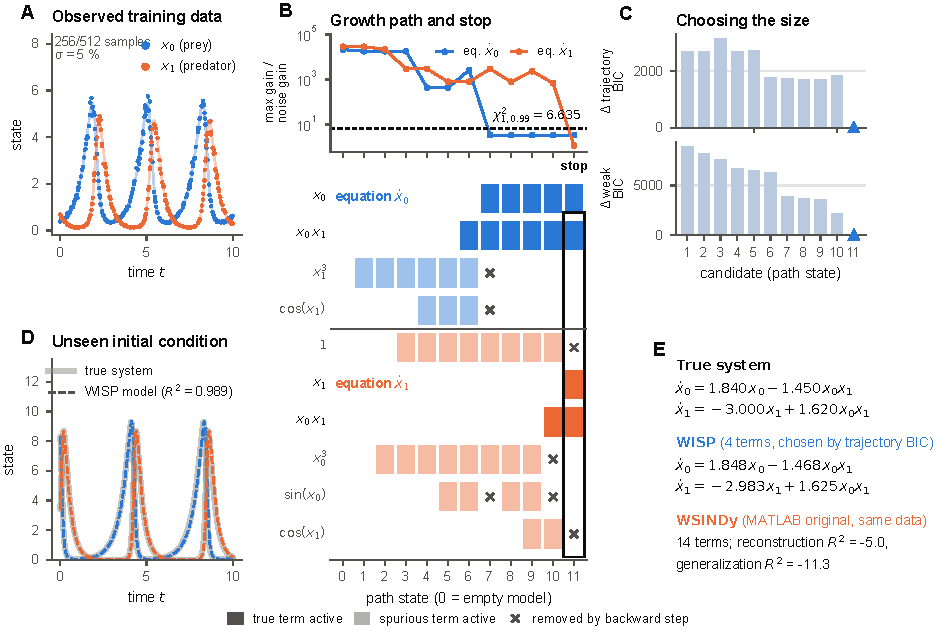
\includegraphics[width=\textwidth]{figures/fig2_example.pdf}
\caption{\textbf{WISP on noisy, irregularly sampled Lotka--Volterra data.} (\textbf{A}) Training data: 256 of 512
samples retained at random, 5\,\% multiplicative noise; faint lines show the clean trajectory, never seen by any
method. (\textbf{B}) The growth path. Bottom: active terms per equation after each forward--backward step (dark: true
terms, light: spurious, crosses: removed by a backward step). Top: the stop statistic of Eq.~\eqref{eq:stop}, the
largest gain-to-noise ratio over the terms not yet in the model; the path ends when both equations fall below
$\chi^2_{1,0.99}$. (\textbf{C}) Size selection among the eleven candidates, each refitted against the trajectory;
differences to the minimum (triangle). Trajectory and weak BIC agree here; they do not in general
(Fig.~\ref{fig:selection}A). (\textbf{D}) Prediction from the unseen initial condition. (\textbf{E}) True and identified
equations.}
\label{fig:example}
\end{figure*}

% ================================================================
\section{Benchmark and protocol}\label{sec:protocol}

\subsection{Systems and data}
ODEBench \cite{dascoli2024} collects 63 ODE systems from Strogatz's textbook \cite{strogatz2015} and the literature,
each with two initial conditions. It spans relaxation, oscillators, bifurcation normal forms, population and epidemic
models, and chaotic three-dimensional flows such as the Lorenz and R\"ossler systems. Following
ref.~\cite{dascoli2024}, each trajectory has 512 samples on $t\in[0,10]$; we integrate them ourselves at tolerance
$10^{-9}$. Each initial condition serves once as training trajectory, and the \emph{other} initial condition is the
test trajectory for generalization, never used for any choice. We evaluate all 63 systems: 51 of dimension 1 and 2 (21
exactly representable, 30 surrogate), which carry every claim, and twelve of dimension 3 and 4, reported descriptively.
Each training trajectory is corrupted by multiplicative Gaussian noise $\sigma\in\{1,2,3,4,5\}\,\%$, with either all
samples kept ($\rho=0$) or half of them removed at random ($\rho=0.5$), the protocol of ref.~\cite{dascoli2024}, in
three independent noise realizations. The headline population is these ten noisy conditions: 60 data sets per system
(10 conditions $\times$ 3 realizations $\times$ 2 training trajectories). Clean data and noise-free subsampled data are
reported separately and never pooled with it. In total WISP is run on 4,284 data sets.

\subsection{Metrics}
A model is \emph{structurally exact} if, after removing coefficients below $\max(10^{-6},10^{-3}\max_j|c_{kj}|)$ in
each equation, its support equals the true support; we report this only on exactly representable systems and also
report the \emph{raw} support without pruning, because the pruned rate alone can hide supersets cleaned up by the rule.
\emph{Reconstruction} and \emph{generalization} hits are $R^2>0.9$ (variance-weighted over components, a divergent
integration counting as a miss) of the model integrated from the clean training and the clean test initial condition,
respectively, against the clean trajectory. The $R^2>0.9$ rate is the metric reported for ODEBench \cite{dascoli2024}.
We report structure and prediction together throughout: on noisy data, a structurally wrong model can still fit its
training trajectory well, and a structurally correct one with poor coefficients can fail to predict.

\subsection{References}
SINDy, Weak-SINDy and Ensemble-SINDy (pySINDy, sequentially thresholded least squares, bagging with 20 models for
E-SINDy) use a degree-3 polynomial plus $\sin/\cos$ library, a superset of $\Theta$, with thresholds
$\lambda\in\{0.01,0.1\}$. WeakIdent \cite{tang2023} is run as the authors' reference code in two arms: with its native
polynomial dictionary of degree 3, and with that dictionary extended by $\sin x_i,\cos x_i$, the only change; its one
user-set parameter, the trimming threshold, is varied over $\tau\in\{0,0.005,0.01,0.02,0.05,0.1,0.2\}$ (authors'
value 0.05). The code does not support four-dimensional systems. WSINDy is run as the unmodified original MATLAB code
\cite{messenger2021mms} with WISP's library; on $\rho=0.5$ the data are interpolated to the uniform grid it requires,
which we found to improve its results substantially.

For every stratum, noise level and metric separately we report each method's \emph{best} threshold, an after-the-fact
choice in its favour: an \emph{oracle-tuned} reference, which no user could select without knowing the truth. WISP
receives no such choice. All reference models are evaluated exactly like WISP's, and every reference result was matched
to WISP's by a hash of the observed data. \todo{v1 data: SINDy, Weak-SINDy, E-SINDy with exactly WISP's library and
$\lambda\in\{10^{-3},\dots,1\}$ (13 values), and ODEFormer (four configurations), both on the same 4,284 data sets.}

\subsection{Statistics}
Data sets of one system are not independent. We therefore treat systems as clusters: a stratum's rate is the mean of its
systems' rates, intervals are 95\,\% percentile cluster-bootstrap intervals over systems \cite{field2007} (10,000
resamples, fixed seed), and paired comparisons use a two-sided sign-flip permutation test on per-system rate
differences, enumerated exactly. The primary family consists of four tests, WISP against WSINDy on exact structure and
on generalization, each in dimension 1 and 2 (exactly representable systems, noisy population), Holm-adjusted
\cite{holm1979} at $\alpha=0.05$. WSINDy is the primary comparator because it is the strongest reference under noise
and the unmodified code of the inventors of weak-form regression; a comparison with ``the best reference per data set''
was rejected because that comparator chooses its method after seeing the result. Every other test is secondary,
reported with its unadjusted $p$, and never described as significant.

\subsection{Pre-registration}
WISP was developed in a sequence of written protocols, each frozen before any number it governs was computed. We
distinguish four kinds of statement.

\emph{Pre-registered decisions.} Adoption rules with a non-inferiority margin of 5 percentage points decided the stop
rule (Eq.~\eqref{eq:stop} replaced a truth-derived cap of six terms per equation, being non-inferior in every decided
stratum and better by 14--17 points on structure), joint initial-state estimation, and the coefficient bound. The
threshold of the stop rule was fixed before its paths were computed; the paths were inspected for whether they contain
the truth before any fit was run, which the protocol records.

\emph{A declared deviation.} The rule for the bound selected $[-10,10]$ over $[-10^3,10^3]$ because dimension-1
generalization was 5.7 points lower under the wider bound, one cell beyond the margin, on three systems whose selected
models were wrong under both bounds and where the narrow bound acted as an accidental regulariser. Structure recovery
was identical under both bounds in every decided stratum, and the narrow bound makes six of the eight
three-dimensional systems infeasible by construction; we adopted $[-10^3,10^3]$ and report both
(Fig.~\ref{fig:ablation}).

\emph{Descriptive analyses.} The breakdown by condition, the per-system comparison, the size-error and
path-versus-selection diagnostics and the cost figures were not governed by any rule and are reported as description.

\emph{Claims.} The final run and, before any of its numbers was computed, the paper's nine claims with their criteria,
statistics and the wording to be used if a criterion fails were frozen in two further protocols; the analysis code was
tested on the subset run before the final data were opened. A data set without a WISP result counts as a miss on every
metric. \todo{data freeze: date, number of finished data sets}

% ================================================================
\section{Results}\label{sec:results}

\ifpreliminary
\noindent\fcolorbox{prelim}{white}{\parbox{\dimexpr\textwidth-2\fboxsep-2\fboxrule}{\sffamily\footnotesize
\textcolor{prelim}{\textbf{Preliminary results.}} Numbers and figures in this section come from a subset run (Q8:
dimensions 1--3, $\sigma\in\{1,5\}\,\%$, $\rho\in\{0,0.5\}$, one noise realization, 590 data sets), evaluated with the
frozen analysis code of the final run. Red numbers are generated and will be replaced automatically by the final run
(Q9: all 63 systems, $\sigma\in\{1,\dots,5\}\,\%$, three realizations, 4,284 data sets); black numbers are final.
Tags [C1]--[C9] mark sentences whose wording depends on a pre-registered claim; on the subset, C3 (structure against
WeakIdent) and C9 (one-dimensional surrogate generalization) fail and are worded accordingly. The ablations
(Fig.~\ref{fig:ablation}) and the stop calibration (Fig.~\ref{fig:calibration}) are final.}}
\vspace{2mm}
\fi

\subsection{Main comparison on noisy data}\label{sec:main}

\begin{figure*}[t]
\centering
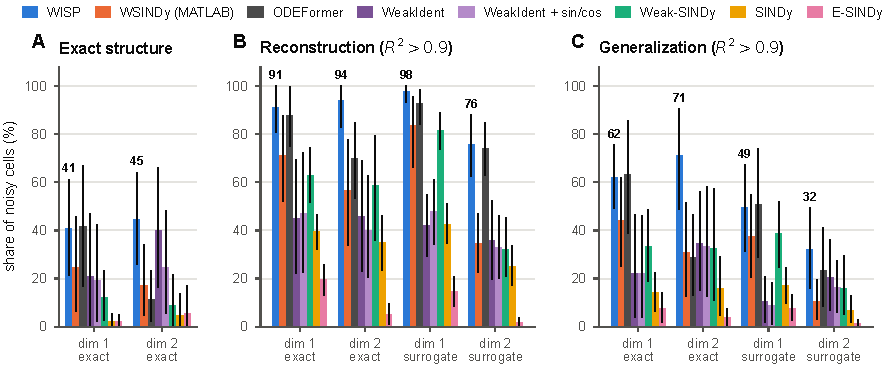
\includegraphics[width=\textwidth]{figures/fig3_main.pdf}
\caption{\textbf{Main comparison on noisy data, dimensions 1 and 2.} Share of the noisy data sets on which each method
recovers the exact structure (\textbf{A}, exactly representable systems only), reconstructs the training trajectory
(\textbf{B}) and predicts the trajectory from the unseen initial condition (\textbf{C}). Whiskers: 95\,\%
cluster-bootstrap intervals over systems (11, 10, 12 and 18 systems per group). References are shown at their best
threshold per group, noise level and metric. \pv{Preliminary: Q8 subset, 408 data sets; WeakIdent not yet shown.}}
\label{fig:main}
\end{figure*}

\paragraph{Structure and prediction on exactly representable systems} On noisy data of exactly representable one- and
two-dimensional systems, WISP recovers the exact structure in \m{WispDimOneExactStructNoisy}\,\% and
\m{WispDimTwoExactStructNoisy}\,\% of data sets (Fig.~\ref{fig:main}A and Table~\ref{tab:main}). The original WSINDy
reaches \m{WsindyDimOneExactStructNoisy}\,\% and \m{WsindyDimTwoExactStructNoisy}\,\% (ratio \m{PrimaryOneRatio} and
\m{PrimaryTwoRatio}; Holm-adjusted $p=\m{PrimaryOnePHolm}$ and $\m{PrimaryTwoPHolm}$), Weak-SINDy
\m{WeakSindyDimOneExactStructNoisy}\,\% and \m{WeakSindyDimTwoExactStructNoisy}\,\%, and SINDy and E-SINDy stay below
\pv{4}\,\%.\claimtag{C1} Without pruning, WISP's raw structure rate is \m{WispDimOneExactRawNoisy}\,\% and
\m{WispDimTwoExactRawNoisy}\,\%; pruned and raw rates are close, so WISP's hits are not produced by the pruning
rule cleaning up supersets. \todo{check this sentence against the Q9 numbers} The same ordering holds for prediction from the unseen initial condition:
\m{WispDimOneExactGenNoisy}\,\% and \m{WispDimTwoExactGenNoisy}\,\% for WISP against \m{WsindyDimOneExactGenNoisy}\,\%
and \m{WsindyDimTwoExactGenNoisy}\,\% for WSINDy (Holm-adjusted $p=\m{PrimaryThreePHolm}$ and $\m{PrimaryFourPHolm}$)
and at most \pv{28.7}\,\% for the pySINDy methods (Fig.~\ref{fig:main}C).\claimtag{C2}

\paragraph{WeakIdent} WeakIdent, which also grows supports in the weak form but selects in regression space, is the
strongest reference on structure. Its predictions from the unseen initial condition stay far behind WISP's
(dimension~2: \m{WeakIdentTrigDimTwoExactGenNoisy}\,\% with $\sin/\cos$, \m{WeakIdentNativeDimTwoExactGenNoisy}\,\%
native, against \m{WispDimTwoExactGenNoisy}\,\%; secondary $p\le\pv{0.016}$ in both dimensions and arms), but on
two-dimensional structure the two methods are not separated: \m{WispDimTwoExactStructNoisy}\,\% against
\m{WeakIdentTrigDimTwoExactStructNoisy}\,\% for the extended arm ($p=\m{VsWeakIdentTrigDimTwoExactStructP}$; WISP
ahead on \m{VsWeakIdentTrigDimTwoExactStructAhead}, tied on \m{VsWeakIdentTrigDimTwoExactStructTied}, behind on
\m{VsWeakIdentTrigDimTwoExactStructBehind} systems), and a difference of
\m{VsWeakIdentNativeDimTwoExactStructDiff} points for the native arm on the systems its dictionary can express
($p=\m{VsWeakIdentNativeDimTwoExactStructP}$). In dimension 1, WISP leads the native arm by
\m{VsWeakIdentNativeDimOneExactStructDiff} points (ahead on \m{VsWeakIdentNativeDimOneExactStructAhead}, behind on
\m{VsWeakIdentNativeDimOneExactStructBehind} systems, $p=\m{VsWeakIdentNativeDimOneExactStructP}$). WISP is therefore
ahead of every reference on generalization, and on structure ahead of every reference except WeakIdent.\claimtag{C3}

\paragraph{Surrogate systems} On surrogate systems, where no exact law exists in the library, WISP's models still
reconstruct the training trajectory in \m{WispDimOneSurrRecNoisy}\,\% and \m{WispDimTwoSurrRecNoisy}\,\% of data sets
and generalize in \m{WispDimOneSurrGenNoisy}\,\% and \m{WispDimTwoSurrGenNoisy}\,\%, ahead of WSINDy in three of the
four comparisons; one-dimensional generalization is not separated (\m{WispDimOneSurrGenNoisy}\,\% vs
\m{WsindyDimOneSurrGenNoisy}\,\%, $p=\m{VsWsindyDimOneSurrGenP}$).\claimtag{C9} Here the library can only approximate
the vector field, and the trajectory criterion chooses the approximation that integrates best rather than the one that
regresses best.

\begin{table*}[t]
\centering\small
\caption{\textbf{Noisy data sets, dimensions 1--2.} Rates in \%, for WISP with the 95\,\% cluster-bootstrap interval
over systems. References at their best threshold per stratum, noise level and metric. WeakIdent: native dictionary /
extended by $\sin/\cos$; native structure is scored only on systems its dictionary can express. Structure (raw): exact
support without the pruning rule. $p$: paired sign-flip test over systems, WISP vs WSINDy; $^\dagger$ primary test,
Holm-adjusted; otherwise secondary, unadjusted. \pv{Preliminary: Q8 subset.}}
\label{tab:main}
\resizebox{\textwidth}{!}{%
\setlength{\tabcolsep}{3.5pt}
\begin{tabular}{@{}llrrrrrrr@{}}
\toprule
 & & \textbf{WISP} & WSINDy & SINDy & Weak-SINDy & E-SINDy & WeakIdent & $p$ \\
 & & & (MATLAB) & & & & native / $+\sin\!/\!\cos$ & \\
\midrule
\multirow{4}{*}{\shortstack[l]{dim 1\\exact}} & structure & \textbf{\m{WispDimOneExactStructNoisy}} \ci{WispDimOneExactStructNoisy} & \m{WsindyDimOneExactStructNoisy} & \m{SindyDimOneExactStructNoisy} & \m{WeakSindyDimOneExactStructNoisy} & \m{EsindyDimOneExactStructNoisy} & \m{WeakIdentNativeDimOneExactStructNoisy} / \m{WeakIdentTrigDimOneExactStructNoisy} & \m{PrimaryOnePHolm}$^\dagger$\\
 & structure (raw) & \textbf{\m{WispDimOneExactRawNoisy}} \ci{WispDimOneExactRawNoisy} & \m{WsindyDimOneExactRawNoisy} & \m{SindyDimOneExactRawNoisy} & \m{WeakSindyDimOneExactRawNoisy} & \m{EsindyDimOneExactRawNoisy} & \m{WeakIdentNativeDimOneExactRawNoisy} / \m{WeakIdentTrigDimOneExactRawNoisy} & \\
 & reconstruction & \textbf{\m{WispDimOneExactRecNoisy}} \ci{WispDimOneExactRecNoisy} & \m{WsindyDimOneExactRecNoisy} & \m{SindyDimOneExactRecNoisy} & \m{WeakSindyDimOneExactRecNoisy} & \m{EsindyDimOneExactRecNoisy} & \m{WeakIdentNativeDimOneExactRecNoisy} / \m{WeakIdentTrigDimOneExactRecNoisy} & \m{VsWsindyDimOneExactRecP}\\
 & generalization & \textbf{\m{WispDimOneExactGenNoisy}} \ci{WispDimOneExactGenNoisy} & \m{WsindyDimOneExactGenNoisy} & \m{SindyDimOneExactGenNoisy} & \m{WeakSindyDimOneExactGenNoisy} & \m{EsindyDimOneExactGenNoisy} & \m{WeakIdentNativeDimOneExactGenNoisy} / \m{WeakIdentTrigDimOneExactGenNoisy} & \m{PrimaryThreePHolm}$^\dagger$\\
\midrule
\multirow{4}{*}{\shortstack[l]{dim 2\\exact}} & structure & \textbf{\m{WispDimTwoExactStructNoisy}} \ci{WispDimTwoExactStructNoisy} & \m{WsindyDimTwoExactStructNoisy} & \m{SindyDimTwoExactStructNoisy} & \m{WeakSindyDimTwoExactStructNoisy} & \m{EsindyDimTwoExactStructNoisy} & \m{WeakIdentNativeDimTwoExactStructNoisy} / \m{WeakIdentTrigDimTwoExactStructNoisy} & \m{PrimaryTwoPHolm}$^\dagger$\\
 & structure (raw) & \textbf{\m{WispDimTwoExactRawNoisy}} \ci{WispDimTwoExactRawNoisy} & \m{WsindyDimTwoExactRawNoisy} & \m{SindyDimTwoExactRawNoisy} & \m{WeakSindyDimTwoExactRawNoisy} & \m{EsindyDimTwoExactRawNoisy} & \m{WeakIdentNativeDimTwoExactRawNoisy} / \m{WeakIdentTrigDimTwoExactRawNoisy} & \\
 & reconstruction & \textbf{\m{WispDimTwoExactRecNoisy}} \ci{WispDimTwoExactRecNoisy} & \m{WsindyDimTwoExactRecNoisy} & \m{SindyDimTwoExactRecNoisy} & \m{WeakSindyDimTwoExactRecNoisy} & \m{EsindyDimTwoExactRecNoisy} & \m{WeakIdentNativeDimTwoExactRecNoisy} / \m{WeakIdentTrigDimTwoExactRecNoisy} & \m{VsWsindyDimTwoExactRecP}\\
 & generalization & \textbf{\m{WispDimTwoExactGenNoisy}} \ci{WispDimTwoExactGenNoisy} & \m{WsindyDimTwoExactGenNoisy} & \m{SindyDimTwoExactGenNoisy} & \m{WeakSindyDimTwoExactGenNoisy} & \m{EsindyDimTwoExactGenNoisy} & \m{WeakIdentNativeDimTwoExactGenNoisy} / \m{WeakIdentTrigDimTwoExactGenNoisy} & \m{PrimaryFourPHolm}$^\dagger$\\
\midrule
\multirow{2}{*}{\shortstack[l]{dim 1\\surrogate}} & reconstruction & \textbf{\m{WispDimOneSurrRecNoisy}} \ci{WispDimOneSurrRecNoisy} & \m{WsindyDimOneSurrRecNoisy} & \m{SindyDimOneSurrRecNoisy} & \m{WeakSindyDimOneSurrRecNoisy} & \m{EsindyDimOneSurrRecNoisy} & \m{WeakIdentNativeDimOneSurrRecNoisy} / \m{WeakIdentTrigDimOneSurrRecNoisy} & \m{VsWsindyDimOneSurrRecP}\\
 & generalization & \textbf{\m{WispDimOneSurrGenNoisy}} \ci{WispDimOneSurrGenNoisy} & \m{WsindyDimOneSurrGenNoisy} & \m{SindyDimOneSurrGenNoisy} & \m{WeakSindyDimOneSurrGenNoisy} & \m{EsindyDimOneSurrGenNoisy} & \m{WeakIdentNativeDimOneSurrGenNoisy} / \m{WeakIdentTrigDimOneSurrGenNoisy} & \m{VsWsindyDimOneSurrGenP}\\
\midrule
\multirow{2}{*}{\shortstack[l]{dim 2\\surrogate}} & reconstruction & \textbf{\m{WispDimTwoSurrRecNoisy}} \ci{WispDimTwoSurrRecNoisy} & \m{WsindyDimTwoSurrRecNoisy} & \m{SindyDimTwoSurrRecNoisy} & \m{WeakSindyDimTwoSurrRecNoisy} & \m{EsindyDimTwoSurrRecNoisy} & \m{WeakIdentNativeDimTwoSurrRecNoisy} / \m{WeakIdentTrigDimTwoSurrRecNoisy} & \m{VsWsindyDimTwoSurrRecP}\\
 & generalization & \textbf{\m{WispDimTwoSurrGenNoisy}} \ci{WispDimTwoSurrGenNoisy} & \m{WsindyDimTwoSurrGenNoisy} & \m{SindyDimTwoSurrGenNoisy} & \m{WeakSindyDimTwoSurrGenNoisy} & \m{EsindyDimTwoSurrGenNoisy} & \m{WeakIdentNativeDimTwoSurrGenNoisy} / \m{WeakIdentTrigDimTwoSurrGenNoisy} & \m{VsWsindyDimTwoSurrGenP}\\
\bottomrule
\end{tabular}}
\end{table*}

\paragraph{Per system} The advantage over WSINDy is not carried by a few systems. Counting each system once, WISP is
ahead on exact structure on \m{PrimaryOneSystemsAhead} of 11 one-dimensional and \m{PrimaryTwoSystemsAhead} of 10
two-dimensional systems and behind on \m{PrimaryOneSystemsBehind} and \m{PrimaryTwoSystemsBehind}; on generalization it
is ahead on \m{PrimaryThreeSystemsAhead} and \m{PrimaryFourSystemsAhead} and behind on \m{PrimaryThreeSystemsBehind} and
\m{PrimaryFourSystemsBehind} (Fig.~\ref{fig:systems}).\claimtag{C4} \todo{Q9: name the systems on which WISP is behind,
and say why.}

\begin{figure}[t]
\centering
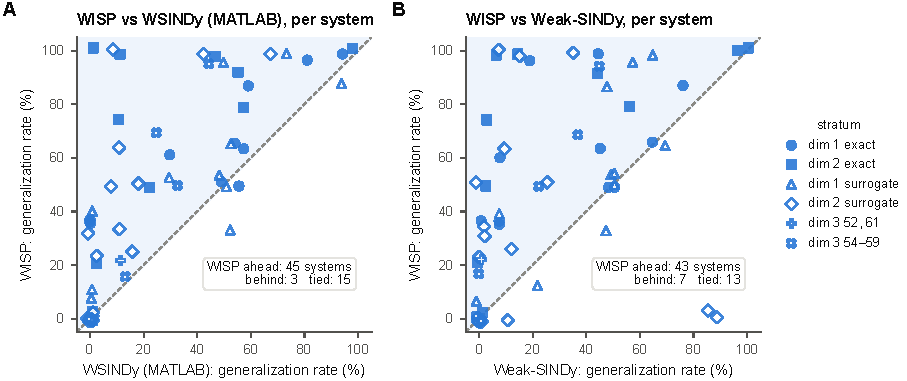
\includegraphics[width=0.78\textwidth]{figures/fig5_systems.pdf}
\caption{\textbf{Per-system comparison of generalization on noisy data.} Each marker is one system (rate over its
noisy data sets); filled markers: exactly representable, open: surrogate. Points above the diagonal favour WISP. Small
jitter added for visibility. \pv{Preliminary: Q8 subset, eight noisy data sets per system (Q9: 60).}}
\label{fig:systems}
\end{figure}

\subsection{The gap opens with noise}\label{sec:conditions}

\begin{figure*}[t]
\centering
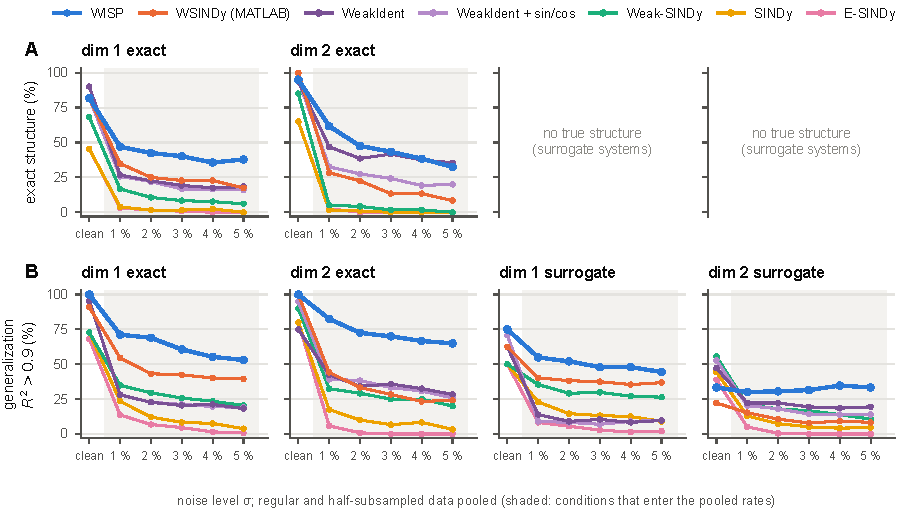
\includegraphics[width=\textwidth]{figures/fig4_conditions.pdf}
\caption{\textbf{Where the advantage comes from.} Exact structure (\textbf{A}) and generalization (\textbf{B}) per data
condition. On clean data (left of each panel) WISP and WSINDy are level on exactly representable systems; the gap
opens with noise and with missing samples. \pv{Preliminary: Q8 subset, two noise levels, one realization; each point
rests on 20--36 data sets.}}
\label{fig:conditions}
\end{figure*}

On clean data WISP and WSINDy are level on exactly representable systems (structure \pv{81.8}\,\% vs \pv{81.8}\,\% in
dimension 1, \pv{95.0}\,\% vs \pv{100}\,\% in dimension 2; Fig.~\ref{fig:conditions}). Pooled over the exactly
representable one- and two-dimensional systems, WISP's structure advantage over WSINDy is \m{GapClean} points on clean
data and \m{GapHighNoise} points at $\sigma=5\,\%$, an opening of \m{GapOpens} points (95\,\% interval
\pv{[\GapOpensLo, \GapOpensHi]}).\claimtag{C5} With 1\,\% noise WSINDy loses about half of its structure hits, while
WISP retains \pv{55--60}\,\%. At 5\,\% noise with half of the samples missing, the hardest condition, WISP still
identifies the exact law in \pv{41}\,\% (dimension 1) and \pv{20}\,\% (dimension 2) of data sets, against \pv{18}\,\%
and \pv{10}\,\% for WSINDy and close to zero for the pySINDy methods. On clean two-dimensional surrogate systems,
Weak-SINDy generalizes better than WISP (\pv{55.6}\,\% vs \pv{33.3}\,\%), a reminder that the advantage is specific to
the noisy regime. \todo{Q9: the trend over $\sigma=1,\dots,5\,\%$ and the effect of $\rho$ separately.}

Two mechanisms plausibly contribute; we did not isolate them experimentally. WSINDy's threshold acts on coefficient
magnitudes, which noise perturbs in every term at once; WISP's stop acts on residual gains referenced to the estimated
noise, so its decision scales with the noise level by construction. And under subsampling, WISP's box test functions
work on the observed times directly, whereas WSINDy needs the data on a uniform grid.

\subsection{Ablations: each component matters, the weak-form start most}\label{sec:ablation}

\begin{figure*}[t]
\centering
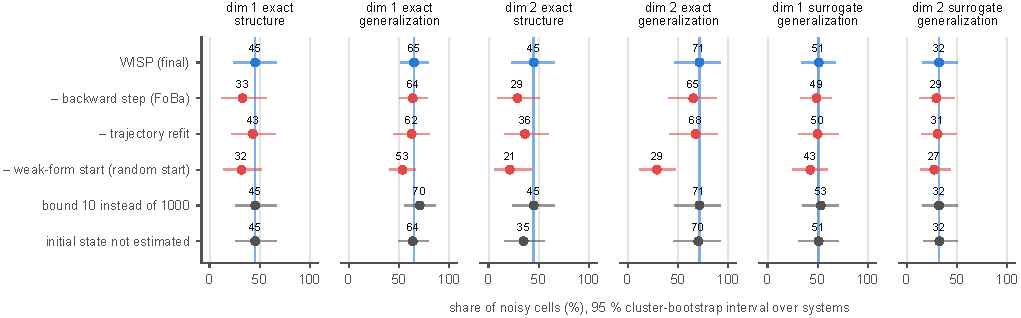
\includegraphics[width=\textwidth]{figures/fig6_ablation.pdf}
\caption{\textbf{Ablations and design alternatives on noisy data} (dimensions 1--2; subset run:
$\sigma\in\{1,5\}\,\%$, $\rho\in\{0,0.5\}$, one realization). Red: one component removed; grey: the two alternatives
decided by pre-registered rules. The vertical line marks the final WISP configuration. Intervals: 95\,\% cluster
bootstrap over systems.}
\label{fig:ablation}
\end{figure*}

Figure~\ref{fig:ablation} removes one component at a time. The ablations were run once, on the subset of the protocol
that fixed the design ($\sigma\in\{1,5\}\,\%$, $\rho\in\{0,0.5\}$, one realization, dimensions 1--2), and are not
repeated on the full grid; all numbers in this subsection refer to that subset.

\emph{Weak-form start.} Replacing the weak-form start by the random start customary in trajectory fitting costs most:
structure recovery falls from 45.0\,\% to 21.2\,\% and generalization from 71.2\,\% to 28.7\,\% on two-dimensional
systems, at the same single optimizer run per candidate. The candidate list is unchanged in this ablation, so the loss
is entirely one of fitting: from a random start, a single optimizer run often does not reach the coefficients that
make a candidate fit, so the BIC compares poorly fitted candidates and can prefer a wrong one.

\emph{Backward steps.} Without backward steps, the forward path accumulates spurious terms that later steps cannot
remove; structure falls by 12--16 points while reconstruction even rises slightly, the signature of over-complete
models that fit the training trajectory but are not the law.

\emph{Trajectory refit.} Selecting among weak-form coefficients without the trajectory refit costs 2--9 points of
structure.

\emph{Bound and initial state.} The coefficient bound and the joint estimation of the initial state change little on
dimension~1; on dimension~2, estimating the initial state raises structure recovery from 35.0\,\% to 45.0\,\%.

\subsection{The trajectory chooses the size; remaining failures lie in the path}\label{sec:selection}

\begin{figure*}[t]
\centering
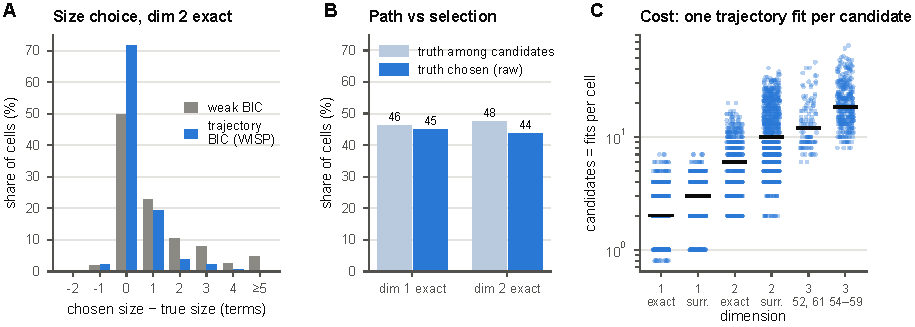
\includegraphics[width=\textwidth]{figures/fig7_selection_cost.pdf}
\caption{\textbf{Selection and cost.} (\textbf{A}) Chosen minus true model size on two-dimensional exactly
representable systems: a BIC on the weak residual over-sizes, the trajectory BIC rarely does. (\textbf{B}) Share of
noisy data sets in which the true structure appears on the growth path, and in which it is chosen. (\textbf{C}) Number of
candidates per noisy data set, which equals the number of trajectory fits; bars mark the median. \pv{Preliminary: Q8
subset.}}
\label{fig:selection}
\end{figure*}

The weak form is a good place to rank terms but a poor place to stop choosing. Choosing the size by a BIC computed on
the weak residual instead of the trajectory over-sizes \m{OversizeWeakDimTwo}\,\% of two-dimensional models
(trajectory BIC: \m{OversizeTrajDimTwo}\,\%; difference interval \pv{[\OversizeDiffLo, \OversizeDiffHi]}
points)\claimtag{C8} and lowers structure recovery from \pv{45.0}\,\% to \pv{32.5}\,\% (Fig.~\ref{fig:selection}A):
the weak residuals are serially correlated, so every additional term looks significant to a criterion that treats them
as independent. On the trajectory, the decision is reliable: whenever the truth appears on the path, it is chosen in
\m{SelectionOnPathNum} of \m{SelectionOnPathDen} noisy data sets (\m{SelectionOnPathShare}\,\%; dimension 1:
\pv{44 of 44}, dimension 2: \pv{35 of 38}; Fig.~\ref{fig:selection}B).\claimtag{C6}

The remaining failures are path failures: in \m{PathFailNum} of the \m{PathFailDen} data sets whose structure is
missed, the truth never appears among the candidates.\claimtag{C7} This locates the room for improvement precisely. A
better selection rule cannot recover these data sets; only a path that visits the true support can. \todo{Q9: describe
the typical path failure---a spurious term that is never removed, or a true term that never enters---by system class.}

\subsection{Cost}\label{sec:cost}

Because the path stops on its own, the candidate list is short: a median of \pv{2, 3, 6 and 9.5} candidates for one-
and two-dimensional exact and surrogate systems, \pv{12 and 19} on dimension 3 (Fig.~\ref{fig:selection}C). Each
candidate costs one trajectory fit, a median of about \pv{3,300} loss evaluations, each of which is one ODE solve. Per
noisy data set this adds up to a median of \pv{4,600} ODE solves on one-dimensional and \pv{14,000} on two-dimensional
exactly representable systems, \pv{39,000} on two-dimensional surrogates and \pv{49,000--158,000} on dimension 3. That
is substantial: WISP is orders of magnitude more expensive than a single sparse regression, which needs no ODE solve for
selection at all. Against searching structures directly on the trajectory it is cheaper: a population-based search on
the same benchmark, our earlier EvoGrow method, ran a median of 410 nonlinear fits per data set even on clean data.

Counts are our measure of cost. As context only, since wall-clock time on a shared cluster depends on the node and its
load: with one CPU core per data set, the recorded solver time per noisy data set has a median of \pv{2.4}\,s
(dimension 1, exact), \pv{6.1}\,s (dimension 2, exact) and \pv{15.7}\,s (dimension 2, surrogate), but a heavy
tail---the 90th percentile is \pv{142}\,s, \pv{2.3}\,h and, on the Lorenz and R\"ossler systems, \pv{31}\,h---driven by
stiff or divergent candidates. A pySINDy fit takes 0.01--0.1\,s per data set on the same cluster. The tail is a
practical limitation: a single candidate whose integration becomes stiff can dominate the cost of a data set.

\subsection{Calibration of the stop}\label{sec:calibration}

\begin{figure}[t]
\centering
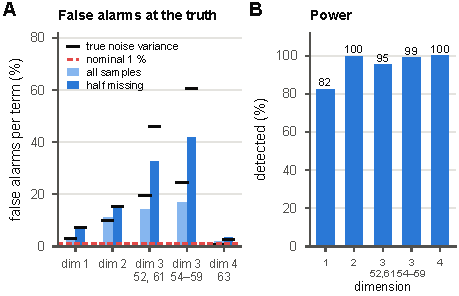
\includegraphics[width=0.62\textwidth]{figures/fig8_calibration.pdf}
\caption{\textbf{Calibration of the $\chi^2$ stop at the true support} (1,800 noisy data sets, 30 exactly representable
systems, $\sigma\in\{1,\dots,5\}\,\%$, three realizations). (\textbf{A}) Share of spurious terms whose gain-to-noise
ratio exceeds $\chi^2_{1,0.99}$; bars with the estimated noise variance, ticks with the true one. (\textbf{B}) Share of
true terms that pass the test when they are the only one missing.}
\label{fig:calibration}
\end{figure}

We probed the $\chi^2$ stop directly, at the true support and without any path (Fig.~\ref{fig:calibration}; separate
protocol, 1,800 noisy data sets of the 30 exactly representable systems, three noise realizations each). It is not
calibrated as a significance test. A spurious term passes the 1\,\% threshold in 5\,\% of cases on dimension 1,
13\,\% on dimension 2 and 23--29\,\% on dimension 3. The excess hardly depends on the noise level, roughly doubles
when half of the samples are missing, and does not shrink when the true noise variance replaces the estimate. This
points to a deterministic error of the weak form---quadrature on coarse or irregular grids and noise entering through
the library---rather than to the noise estimator. At the same time the test has high power: a missing true term is
detected in 82--100\,\% of cases.

The stop therefore errs on the side of letting the path run past the truth, and the trajectory BIC then cuts it
back---which is the division of labour WISP is built on. A sharper stop would shorten paths and lower cost; in our data
the excess false alarms were largely absorbed by the trajectory selection, but we have not shown that better
calibration would leave correctness unchanged.

\subsection{Three- and four-dimensional systems}\label{sec:dim3}

\begin{table}[t]
\centering\small
\caption{\textbf{Three-dimensional exactly representable systems, noisy data.} Hits out of $n$ noisy data sets for
structure / reconstruction / generalization. Weak-SINDy reached 0 structure hits on every system. \pv{Preliminary: Q8
subset, eight noisy data sets per system (Q9: 60).}}
\label{tab:dim3}
\setlength{\tabcolsep}{5pt}
\ifpreliminary\color{prelim}\fi
\begin{tabular}{@{}rlccc@{}}
\toprule
 & system & $n$ & \textbf{WISP} & WSINDy \\
\midrule
52 & Maxwell--Bloch & 8 & 0 / \textbf{7} / 0 & 0 / 2 / 0\\
54 & Lorenz, periodic & 8 & \textbf{3} / \textbf{7} / \textbf{4} & 2 / 3 / 2\\
55 & Lorenz, complex periodic & 7 & 1 / 0 / 0 & \textbf{2} / 0 / 0\\
56 & Lorenz, chaotic & 8 & 1 / 0 / 0 & \textbf{2} / 0 / 0\\
57 & R\"ossler, fixed point & 8 & 0 / \textbf{4} / 0 & 0 / 0 / \textbf{2}\\
58 & R\"ossler, periodic & 8 & \textbf{5} / \textbf{7} / \textbf{6} & 0 / 5 / 4\\
59 & R\"ossler, chaotic & 8 & \textbf{3} / \textbf{7} / \textbf{5} & 1 / 1 / 3\\
61 & Chen--Lee & 7 & 4 / \textbf{2} / \textbf{3} & 4 / 1 / 1\\
\midrule
 & total & 62 & \textbf{17} / \textbf{34} / \textbf{18} & 11 / 12 / 12\\
\bottomrule
\end{tabular}
\end{table}

Table~\ref{tab:dim3} reports the eight exactly representable three-dimensional systems, \pv{62} noisy data sets. WISP
recovers the exact structure in \pv{17 of 62} (WSINDy \pv{11}, all pySINDy methods \pv{0}) and reconstructs the
trajectory in \pv{34} (WSINDy \pv{12}). The chaotic and complex-periodic Lorenz regimes (55, 56) are hard for every
method: trajectory losses lose their meaning beyond a few Lyapunov times, so a trajectory criterion cannot reward the
correct model over a wrong one once both have decorrelated from the data. On Maxwell--Bloch (52), WISP reconstructs the
trajectory in \pv{7 of 8} data sets but never isolates the exact law. On clean data WSINDy recovers more
three-dimensional structures than WISP (\pv{11 of 12 vs 9 of 12} on systems 54--59). These counts rest on eight systems
and are reported, not used for any claim. \todo{Q9: add the two three-dimensional surrogate and the two
four-dimensional systems; Maxwell--Bloch and Chen--Lee reported apart from the Lorenz and R\"ossler regimes.}

% ================================================================
\section{Discussion}\label{sec:discussion}

\subsection{Ranking and deciding are different problems}
WISP rests on one observation: ranking candidate terms and deciding on a model are different problems, and they are
best solved in different spaces. In the weak form, the question ``which term explains most of what is left?'' has a
linear, derivative-free answer, and the question ``is that more than noise?'' has a closed-form reference value. On the
trajectory, the question ``does this model, integrated, reproduce the data?'' is answered directly, and the weak
coefficients keep that answer to one fit per candidate. Neither half is new on its own---orthogonal forward regression
\cite{billings1989}, FoBa \cite{zhang2011}, weak formulations \cite{schaeffer2017,messenger2021mms}, simulation-based
model selection \cite{mangan2017,piroddi2003} and weak-form starting values for trajectory fits \cite{bortz2023} are all
established---but their combination behaves very differently from each component. Selection in the weak form alone
over-sizes (Fig.~\ref{fig:selection}A), and trajectory search from random starts fails to find even known structures
(Fig.~\ref{fig:ablation}); together they roughly double structure recovery under noise compared with
WSINDy.\claimtag{C1}

The comparison with WeakIdent isolates what the trajectory adds. Both methods grow supports in the weak form and find
exact two-dimensional structures at comparable rates, but WISP's models predict from an unseen initial condition far
more often (\m{WispDimTwoExactGenNoisy}\,\% vs at most \m{WeakIdentTrigDimTwoExactGenNoisy}\,\%).\claimtag{C3} A growth
path in the weak form is thus enough to find the terms; deciding the model and its coefficients on the trajectory is
what makes it predict. For a dynamical model, the second property matters at least as much as the first: a model is
used by integrating it.

\subsection{Where the remaining errors sit}
The most useful finding for future work may be where the remaining errors sit. When the true law is among WISP's
candidates, the trajectory criterion picks it in \m{SelectionOnPathNum} of \m{SelectionOnPathDen} noisy data sets on
one- and two-dimensional systems (Fig.~\ref{fig:selection}B).\claimtag{C6} Under noise, selection is therefore
essentially solved for these systems, and recovery is bounded by the candidate generator: in about \pv{half} of the data
sets the truth never appears on the path.\claimtag{C7} This turns the question of how to improve equation discovery
from noisy data into a sharper one: how to generate a short candidate list that contains the truth more often. The
answer does not need to change the selection step at all.

\subsection{A threshold that follows the noise}
Sparse regression needs a threshold, and the right threshold depends on noise and scale; in our comparison the
references were oracle-tuned---granted their best threshold \emph{after} seeing the results---and still fell behind on
generalization.\claimtag{C3} WISP's path ends where its gain becomes indistinguishable from noise, with noise estimated
from the data. Replacing a truth-derived cap by this rule shortened the paths by half and improved structure recovery by
14--17 points. The calibration shows that this stop is liberal, but in a two-stage method a liberal stop is the safe
error: a path that runs past the truth costs fits, a path that stops before it costs the result.

\subsection{Practical guidance}
WISP is worth its cost when the data are noisy or irregularly sampled, when only one trajectory is available, and when
the identified model will be integrated---for prediction, simulation or control design. On clean, uniformly sampled
data WSINDy recovers the same structures at a fraction of the cost, and a sparse regression remains the first thing to
try. The library has to be chosen by the user, as in every library method; WISP's stop and selection adapt to its size,
but they cannot find terms that are not in it. The noise estimator assumes that the dynamics are smooth on the scale of its nine-point local fits; where the
sampling is too coarse for that, the estimate, and with it the stop, degrades. For
systems with more than a handful of states, the cost of the trajectory fits and the reach of the trajectory criterion on
chaotic dynamics are the limiting factors (Sect.~\ref{sec:dim3}).

\subsection{Limitations}
The library is fixed and polynomial-trigonometric; 33 of 63 ODEBench systems have no exact representation in it, and
WISP's generalization on two-dimensional surrogate systems (\m{WispDimTwoSurrGenNoisy}\,\%) remains low in absolute
terms, as for every method we tested. All evidence comes from one training trajectory per data set, the setting of
ODEBench; on chaotic systems this caps what any trajectory-based criterion can do. The $\chi^2$ stop is a first-order
approximation that ignores noise in the library columns and quadrature error; it is liberal by a factor of 5--30
(Fig.~\ref{fig:calibration}); in our data this cost fits rather than correctness, because the trajectory selection
absorbed most of the excess. We therefore do not call it a significance test but a heuristic that errs in the safe
direction. We did not raise the threshold to match the observed false-alarm rate, because that would tune a constant on
the benchmark; on one-dimensional systems, where 18\,\% of missing true terms stay below the threshold, the opposite
error also occurs. A size rule based on the trajectory loss plus an absolute complexity penalty recovered slightly more
two-dimensional structures than the BIC (\pv{47.5}\,\% vs \pv{45.0}\,\%); it was not adopted because the protocol fixed
the BIC beforehand. The ablations rest on a subset of two noise levels and one realization, and dimensions 3 and 4 on
twelve systems. The cost has a heavy tail driven by stiff candidates. Finally, our comparison covers the SINDy family
and WeakIdent \todo{v1 data: and ODEFormer, run on the same data}; genetic-programming PySR \cite{cranmer2023} reports
generalization rates on ODEBench of the same order as the references here, but on different data, and we do not compare
against it numerically.

% ================================================================
\section{Conclusions}\label{sec:conclusions}

WISP identifies sparse ODEs from one noisy, possibly irregularly sampled trajectory by growing the model in the weak form
and deciding on it against the trajectory. On ODEBench under 1--5\,\% noise it roughly doubles exact structure recovery
on one- and two-dimensional systems compared with WSINDy and predicts from unseen initial conditions markedly more often
than every reference, each granted its best threshold after the fact.\claimtag{C1--C3} Its components are established;
what is new is the division of labour between the two spaces, a stop referenced to the noise instead of a sparsity
threshold, and the evidence that, once the truth is on the path, the trajectory criterion nearly always finds it. The
next steps follow from where the errors sit: a calibrated stop whose noise floor includes the quadrature error and the
noise propagated through the library, and better paths---beam variants that keep more than one support alive, or
several trajectories at once. Both can be added without giving up the property that makes WISP easy to use: every
component can be stated in one sentence, and none was tuned on the benchmark.

% ================================================================
\section*{Declarations}
\addcontentsline{toc}{section}{Declarations}

\paragraph{Funding} \todo{funding statement (SCCH / COMET programme wording, project number), to be supplied}

\paragraph{Competing interests} The authors declare that they have no competing interests. \todo{all authors to confirm}

\paragraph{Author contributions} \todo{CRediT statement, e.g. D.J.: conceptualization, methodology, software,
investigation, writing; S.M.W., M.A.: supervision, writing---review and editing}

\paragraph{Data availability} ODEBench is publicly available \cite{dascoli2024}. The per-cell results of WISP and every
reference, all protocols with their version history, and the scripts that produce every number and figure in this
article are provided to the reviewers at submission and will be released publicly upon publication.

\paragraph{Code availability} The WISP implementation is provided to the reviewers at submission and will be released
publicly as an open-source package upon publication.

\paragraph{Acknowledgements} Computations were performed on the Orion cluster of SCCH.

% ================================================================
\begin{appendices}

\section{Implementation details}\label{app:impl}

\paragraph{Weak design} For $L\in\{1,2,4,8,16\}$ and every start index $a$, row $(L,a)$ has target
$x_k(t_{a+L})-x_k(t_a)$ and design $\int_{t_a}^{t_{a+L}}\theta_j\,dt$ by the trapezoidal rule on the observed times
(about $2{,}530$ rows for 512 samples). Columns are not centred; the constant is an ordinary column. Least squares uses an
orthogonal factorization on unit-norm columns; $\SSE$ is scale invariant.

\paragraph{Noise estimate and stop} For each component and observed point $i$, a cubic is fitted by least squares to the
nine observed points centred on $i$ (shifted at the edges); its residual at $i$ is divided by $\sqrt{1-h_{ii}}$ with
leverage $h_{ii}$, squared, and averaged over the 21 points centred on $i$.
$C_k=D\,\mathrm{diag}(\hat\sigma^2_{k,\cdot})D^\top$ with the end-point incidence matrix $D$; $F_k(S)$ is computed
through a thin SVD of the unit-normalized columns $S$ without forming $C_k$. A non-positive expected noise gain counts
as significant. The path also ends when the best available gain is non-positive, when a backward step would revisit a
model, or when the full library is active.

\paragraph{Trajectory fit} ODEs are integrated with Tsitouras' 5(4) Runge--Kutta pair \cite{tsitouras2011}
(DifferentialEquations.jl \cite{rackauckas2017}, absolute and relative tolerance $10^{-6}$); the loss is minimized by
BFGS (Optim.jl \cite{mogensen2018}, via Optimization.jl) with at most 200 iterations and 20,000 loss evaluations, one
attempt. BFGS itself is unconstrained; the coefficients enter the ODE clipped to $[-10^3,10^3]$, the initial state
unclipped. Failed or divergent fits are never selected.

\paragraph{Evaluation} Models are integrated from the clean initial conditions on the clean 512-point grid. $R^2$ is
variance weighted over components; a divergent integration counts as a miss. Reference models are integrated with
DOP853 at the same evaluation settings. Each reference row was matched to WISP's row by a hash of the observed data.

\paragraph{Reference implementations} SINDy: pySINDy, second-order finite differences. Weak-SINDy: pySINDy weak library.
E-SINDy: pySINDy ensemble optimizer, bagging, 20 models, median aggregation. WSINDy: original MATLAB code (version used
in ref.~\cite{messenger2021mms}), library identical to $\Theta$; MATLAB R2026b. WeakIdent: authors' reference code, ODE
mode, polynomial dictionary of degree 3, in a second arm extended by $\sin x_i,\cos x_i$ (the arm without them
reproduces the native arm bit-identically); test functions and sparsity limit are derived from the data by the code.
For every reference with a threshold we evaluated all values and report, per stratum $\times$ noise level $\times$
metric, the best one; the single best value per stratum and the whole threshold curve are given in the supplement
\todo{supplement}.

\section{Calibration protocol}\label{app:calibration}
For every noisy data set of the 30 exactly representable systems (both training initial conditions,
$\sigma\in\{0.01,\dots,0.05\}$, $\rho\in\{0,0.5\}$, three realizations) and every equation, the gain-to-noise ratio of
Eq.~\eqref{eq:stop} was computed at the true support $S^*$ for every $j\notin S^*$ (false alarms) and for every true
term $i$ added to $S^*\setminus\{i\}$ (power), once with the estimated and once with the true per-point noise variance
$(\sigma x_{\mathrm{clean}}(t_i))^2$. No path, fit or simulation is involved. The protocol was frozen before the first
number; the analysis is descriptive and changed nothing in WISP.

\section{Pre-registered protocols}\label{app:protocols}
The protocols, the adoption rules and the decision records are part of the code repository; each records its freeze
date before the governed computation. All runs execute in one container image per protocol on a Kubernetes cluster;
every record carries a settings fingerprint and the hash of its input data. \todo{supplement: list of protocols with
freeze dates and the decision each governed.}

\end{appendices}

% ================================================================
\small
\begin{thebibliography}{99}\setlength{\itemsep}{1pt}\setlength{\parskip}{0pt}
\bibitem{bongard2007} Bongard J, Lipson H (2007) Automated reverse engineering of nonlinear dynamical systems. Proc Natl Acad Sci USA 104(24):9943--9948
\bibitem{schmidt2009} Schmidt M, Lipson H (2009) Distilling free-form natural laws from experimental data. Science 324(5923):81--85
\bibitem{cranmer2023} Cranmer M (2023) Interpretable machine learning for science with PySR and SymbolicRegression.jl. arXiv:2305.01582
\bibitem{brunton2016} Brunton SL, Proctor JL, Kutz JN (2016) Discovering governing equations from data by sparse identification of nonlinear dynamical systems. Proc Natl Acad Sci USA 113(15):3932--3937
\bibitem{rudy2017} Rudy SH, Brunton SL, Proctor JL, Kutz JN (2017) Data-driven discovery of partial differential equations. Sci Adv 3(4):e1602614
\bibitem{champion2019} Champion K, Lusch B, Kutz JN, Brunton SL (2019) Data-driven discovery of coordinates and governing equations. Proc Natl Acad Sci USA 116(45):22445--22451
\bibitem{kaheman2020} Kaheman K, Kutz JN, Brunton SL (2020) SINDy-PI: a robust algorithm for parallel implicit sparse identification of nonlinear dynamics. Proc R Soc A 476(2242):20200279
\bibitem{desilva2020} de Silva BM, Champion K, Quade M, Loiseau JC, Kutz JN, Brunton SL (2020) PySINDy: a Python package for the sparse identification of nonlinear dynamical systems from data. J Open Source Softw 5(49):2104
\bibitem{kaptanoglu2022} Kaptanoglu AA, et al.\ (2022) PySINDy: a comprehensive Python package for robust sparse system identification. J Open Source Softw 7(69):3994
\bibitem{fasel2022} Fasel U, Kutz JN, Brunton BW, Brunton SL (2022) Ensemble-SINDy: robust sparse model discovery in the low-data, high-noise limit, with active learning and control. Proc R Soc A 478(2260):20210904
\bibitem{tibshirani1996} Tibshirani R (1996) Regression shrinkage and selection via the lasso. J R Stat Soc B 58(1):267--288
\bibitem{champion2020sr3} Champion K, Zheng P, Aravkin AY, Brunton SL, Kutz JN (2020) A unified sparse optimization framework to learn parsimonious physics-informed models from data. IEEE Access 8:169259--169271
\bibitem{bertsimas2023} Bertsimas D, Gurnee W (2023) Learning sparse nonlinear dynamics via mixed-integer optimization. Nonlinear Dyn 111(7):6585--6604
\bibitem{schaeffer2017} Schaeffer H, McCalla SG (2017) Sparse model selection via integral terms. Phys Rev E 96(2):023302
\bibitem{reinbold2020} Reinbold PAK, Gurevich DR, Grigoriev RO (2020) Using noisy or incomplete data to discover models of spatiotemporal dynamics. Phys Rev E 101(1):010203
\bibitem{messenger2021mms} Messenger DA, Bortz DM (2021) Weak SINDy: Galerkin-based data-driven model selection. Multiscale Model Simul 19(3):1474--1497
\bibitem{messenger2021jcp} Messenger DA, Bortz DM (2021) Weak SINDy for partial differential equations. J Comput Phys 443:110525
\bibitem{bortz2023} Bortz DM, Messenger DA, Dukic V (2023) Direct estimation of parameters in ODE models using WENDy: weak-form estimation of nonlinear dynamics. Bull Math Biol 85:110
\bibitem{tang2023} Tang M, Liao W, Kuske R, Kang SH (2023) WeakIdent: weak formulation for identifying differential equation using narrow-fit and trimming. J Comput Phys 483:112069
\bibitem{billings1989} Billings SA, Chen S, Korenberg MJ (1989) Identification of MIMO non-linear systems using a forward-regression orthogonal estimator. Int J Control 49(6):2157--2189
\bibitem{chen1989} Chen S, Billings SA, Luo W (1989) Orthogonal least squares methods and their application to non-linear system identification. Int J Control 50(5):1873--1896
\bibitem{billings2013} Billings SA (2013) Nonlinear system identification: NARMAX methods in the time, frequency, and spatio-temporal domains. Wiley, Chichester
\bibitem{tropp2007} Tropp JA, Gilbert AC (2007) Signal recovery from random measurements via orthogonal matching pursuit. IEEE Trans Inf Theory 53(12):4655--4666
\bibitem{zhang2011} Zhang T (2011) Adaptive forward-backward greedy algorithm for learning sparse representations. IEEE Trans Inf Theory 57(7):4689--4708
\bibitem{schwarz1978} Schwarz G (1978) Estimating the dimension of a model. Ann Stat 6(2):461--464
\bibitem{burnham2002} Burnham KP, Anderson DR (2002) Model selection and multimodel inference: a practical information-theoretic approach, 2nd edn. Springer, New York
\bibitem{mangan2017} Mangan NM, Kutz JN, Brunton SL, Proctor JL (2017) Model selection for dynamical systems via sparse regression and information criteria. Proc R Soc A 473(2204):20170009
\bibitem{piroddi2003} Piroddi L, Spinelli W (2003) An identification algorithm for polynomial NARX models based on simulation error minimization. Int J Control 76(17):1767--1781
\bibitem{ramsay2007} Ramsay JO, Hooker G, Campbell D, Cao J (2007) Parameter estimation for differential equations: a generalized smoothing approach. J R Stat Soc B 69(5):741--796
\bibitem{dascoli2024} d'Ascoli S, Becker S, Mathis A, Schwaller P, Kilbertus N (2024) ODEFormer: symbolic regression of dynamical systems with transformers. In: International Conference on Learning Representations (ICLR)
\bibitem{strogatz2015} Strogatz SH (2015) Nonlinear dynamics and chaos, 2nd edn. Westview Press, Boulder
\bibitem{field2007} Field CA, Welsh AH (2007) Bootstrapping clustered data. J R Stat Soc B 69(3):369--390
\bibitem{holm1979} Holm S (1979) A simple sequentially rejective multiple test procedure. Scand J Stat 6(2):65--70
\bibitem{tsitouras2011} Tsitouras Ch (2011) Runge--Kutta pairs of order 5(4) satisfying only the first column simplifying assumption. Comput Math Appl 62(2):770--775
\bibitem{rackauckas2017} Rackauckas C, Nie Q (2017) DifferentialEquations.jl -- a performant and feature-rich ecosystem for solving differential equations in Julia. J Open Res Softw 5(1):15
\bibitem{mogensen2018} Mogensen PK, Riseth AN (2018) Optim: a mathematical optimization package for Julia. J Open Source Softw 3(24):615
\end{thebibliography}

\end{document}
